\documentclass[12pt, a4paper]{article}

\usepackage[utf8]{inputenc}
\usepackage{color}
\usepackage{multicol}
\usepackage{graphicx}
\usepackage{animate}
\usepackage{subfigure,color,soul}

\usepackage[round]{natbib}
\usepackage{array, multirow, makecell}
\setcellgapes{1pt}
\makegapedcells
\newcolumntype{R}[1]{>{\centering\arraybackslash }b{#1}}
\newcolumntype{L}[1]{>{\centering\arraybackslash }b{#1}}
\newcolumntype{C}[1]{>{\centering\arraybackslash }b{#1}}

\usepackage{stmaryrd}
\usepackage{dsfont}
\usepackage{amsmath}
\usepackage{xcolor}         % pour d\'efinir plus de couleurs
\usepackage{animate}
\usepackage{ulem}
\usepackage{url}
%\usepackage{multimedia}
\usepackage{geometry}

\geometry{hmargin=2cm,vmargin=2cm}
\usepackage{amssymb}
\usepackage[english,french]{babel}
\usepackage{hyperref}
\usepackage[T1]{fontenc}
\usepackage{eurosym}
\usepackage{blindtext}

\newcommand{\itemmarker}{{\small\textbullet}}
\newcommand{\ratingmarker}{\faCircle}

\numberwithin{figure}{section} % Commande de BibiFlo pour faire des trucs super géniaux qui pètent leur race dans LOF



%---------------------------------------------------------------------------------------------------------------------------------------------------%

\begin{document}




    \begin{titlepage}
         \begin{center}
            \Huge{\textbf{Manuel d'Utilisation :}}
            
            \Huge{\textbf{Montage et programmation d'une main robotisée}}
            
            \vspace{2cm}
                \LARGE{\textbf{Albaladejo Joris}}
                
                \vspace{2cm}
                \Large {\textbf{ Association 1901 \textit{Robots !}}}
                
                \vspace{1cm}
                \Large{\textbf{Janvier 2021\\
                -\\
                Février 2021\\
                }}
                
                \vspace{3cm}
                
\includegraphics{Images_main/logo_asso.png}
        \end{center}
    \end{titlepage}

%---------------------------------------------------------------------------------------------------------------------------------------------------%

\newpage

\thispagestyle{empty}
        \tableofcontents
        
        \newpage
        \listoffigures
        




%---------------------------------------------------------------------------------------------------------------------------------------------------%

\newpage

\section{Introduction à la CAO \& à l'impression 3D}

\subsection{Qu'est-ce que la CAO ?}

\begin{flushleft}
    La CAO, ou Conception Assistée par Ordinateur (Computer Aided Design en anglais) est l'ensemble des logiciels et des techniques de modélisation géométriques permettant de simuler et de visualiser la structure et le fonctionnement d'un objet en prévision de sa fabrication. De nos jours elle est couramment utilisée dans l'industrie.\\
    Il existe de nombreux logiciels de CAO, certains adaptés à l'électronique, d'autres à la mécanique, à l'industrie automobile, etc..\\ \href{https://all3dp.com/1/best-free-3d-modeling-software-for-beginners/}{Ici}, un lien regroupant une liste de logiciels de CAO gratuits.\\\vspace{0.2cm}
    
\includegraphics[width=30pt,height=30pt]{Déroulé/Jour_1/idée.png}
    \textbf{\large Astuce : }\textbf{\textit{\large Certains logiciels de CAO payants proposent une licence gratuite ou à bas coût pour les étudiants. (Par exemple SolidWorks developpé par la société Dassault ou encore la suite de logiciels Autodesk)}}

\subsection{Qu'est-ce que l'impression 3D ?}

     L'impression 3D est une technique permettant de fabriquer de manière automatisée et reproductible des objets en trois dimensions.\\
     Elle permet de réaliser une pièce par superpositions successives de fines couches de matière (ALM : Additive Layer Manufacturing en anglais).\\
     Il existe différents types d'imprimantes, utilisant des techniques de dépôt de matière spécifiques. De plus, il y a également plusieurs types de matériaux pour faire de l'impression 3D.\vspace{0.2cm}
     
     \begin{multicols}{2}
     
\includegraphics[width=60pt,height=60pt]{Déroulé/Jour_1/Manuel d'utilisation/Images/6.jpg}
     
     \columnbreak
     
     \textbf{Attention : }\textbf{\textit{Il faut se renseigner sur le (ou les) matériau(x) supporté(s) par l'imprimante que l'on va utiliser. En effet chaque imprimante a ses spécificités.}}
     \end{multicols}
\end{flushleft}

\subsection{Où trouver les ressources pour faire de l'impression 3D ?}

\subsubsection{Quels sites et/ou logiciels utiliser ?}
\begin{flushleft}
    Il existe de nombreux sites internet où l'on peut trouver des fichiers 3D en open source déposés et conçus par d'autres utilisateurs. Ci-dessous, quelques exemples et les liens vers ces sites.\\
\end{flushleft}

\begin{flushleft}
    \begin{figure}[!h]
        \begin{center}
        
\includegraphics[width=100pt,height=100pt]{Déroulé/Jour_1/logo_grabcad.png}
        
\includegraphics[width=100pt,height=100pt]{Déroulé/Jour_1/logo_cults3D.png}
        
\includegraphics[width=100pt,height=100pt]{Déroulé/Jour_1/logo_Thingiverse.png}
        
\includegraphics[width=100pt,height=100pt]{Déroulé/Jour_1/logo_instructables.png}\\
        \caption[Sites de modèles 3D]{Logos de quelques sites de modèles 3D}
        \label{fig:my_label}
        \end{center}
    \end{figure}
    
    
    \vskip0.5cm
    \begin{tabular}{|l|l|}
        \hline Site & Lien\\
        \hline Grabcad & \url{https://grabcad.com/library}\\
        \hline Cults3D & \url{https://grabcad.com/library}\\
        \hline Thingiverse & \url{https://www.thingiverse.com/}\\
        \hline Instructables & \url{https://www.instructables.com/workshop/3d-printing/projects/}\\
        \hline
    \end{tabular}\\\vskip0.5cm
    \href{https://all3dp.com/fr/1/ficher-stl-3d-gratuit-modele-3d-imprimante-3d/}{Ici}, le lien d'un article répertoriant plus de plateformes pour trouver des fichiers 3D.\\\vspace{0.2cm}
    
    \begin{multicols}{2}
    
\includegraphics[width=60pt,height=60pt]{Déroulé/Jour_1/Manuel d'utilisation/Images/6.jpg}
    
    \columnbreak
    
    \textbf{\large Attention : }\textbf{\textit{\large Certains de ces sites nécessitent la création d'un compte pour pouvoir télécharger les modèles, et certains modèles peuvent être payants.}}
    \end{multicols}
\end{flushleft}

\begin{flushleft}
    Trouver son modèle c'est bien... L'imprimer c'est mieux ! \textbf{Mais comment faire pour imprimer son fichier 3D ?}\\
    Pour pouvoir effectuer une impression 3D il faut passer via un logiciel dit "Trancheur 3D" (ou Slicer 3D en anglais).\vspace{0.4cm}
    
    \textbf{Mais qu'est-ce qu'un trancheur 3D ?}\\
    Un trancheur permet de calculer les couches qui seront imprimées ce qui revient à découper l'objet en intervalles de hauteur réguliers. De nombreux paramètres peuvent être ajustés afin d'adapter l'impression à l'imprimante 3D et à la qualité souhaitée de l'objet. Ils sont généralement identiques d'un logiciel à l'autre, nous les aborderons donc lors de la prise en main d'\textit{Ultimaker Cura}.
    
    \href{https://all3dp.com/fr/1/meilleur-slicer-3d-logiciel-decoupe-impression-3d/}{Ici}, le lien d'un article regroupant les trancheurs 3D utilisés le plus couramment.\\\vspace{0.2cm}
    
    \begin{multicols}{2}
    
\includegraphics[width=60pt,height=60pt]{Déroulé/Jour_1/Manuel d'utilisation/Images/6.jpg}
    
    \columnbreak
    
    \textbf{\large Attention : }\textbf{\textit{\large Certains de ces logiciels possèdent différentes versions. Certaines gratuites, d'autres payantes.}}
    \end{multicols}
\end{flushleft}

\subsubsection{Ce que l'on utilise pour cet atelier}
\begin{multicols}{2}
    
\includegraphics[width=50pt,height=50pt]{Déroulé/Jour_1/logo_cura.png}\\
    \columnbreak
    \begin{flushleft}
        Au cours de cet atelier, nous allons uniquement utiliser le logiciel \textit{Ultimaker Cura} pour visualiser puis imprimer les différentes pièces de la main.
    \end{flushleft}
\end{multicols}

%provisoire
\newpage

\begin{flushleft}
    \textbf{La source des fichiers utilisés pour imprimer la main :}
    
    Toutes les pièces 3D que nous utilisons viennent du projet de \href{https://www.instructables.com/3D-Printed-Robotic-Hand/}{TechMartian} (cliquer sur le pseudo pour accéder à la page de son projet et aux fichiers d'impression 3D) et sont également disponibles sur le site de \href{https://www.association-robots.com/}{\textit{Robots!}}. Ci-dessous, une photographie du modèle final qu'il a réalisé :\\
    
    \begin{figure}[!h]
        \centering
        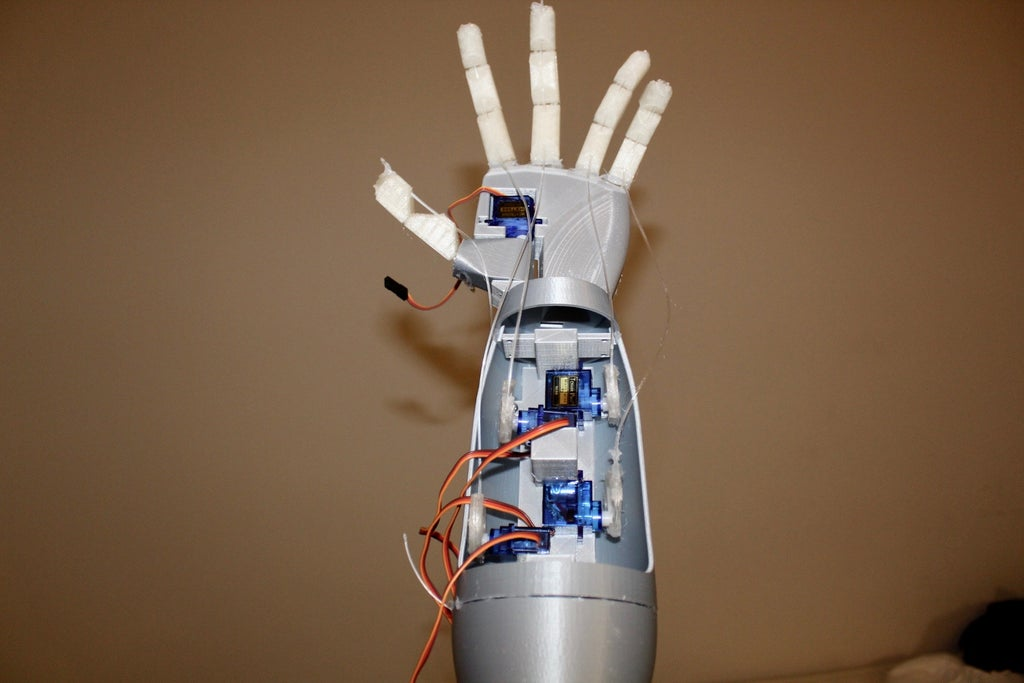
\includegraphics[width=200pt]{Déroulé/Jour_1/modèle_choisi.jpg}
        \caption[Projet de TechMartian]{Main robotique réalisée par TechMartian}
        \label{fig:my_label}
    \end{figure}
\end{flushleft}

\begin{flushleft}
     Au cours de l'atelier nous allons pas à pas monter et programmer notre modèle.
     Ci-dessous, une photo du modèle auquel nous arriverons à la fin de l'atelier:\\
    
    \begin{figure}[!h]
        \centering
        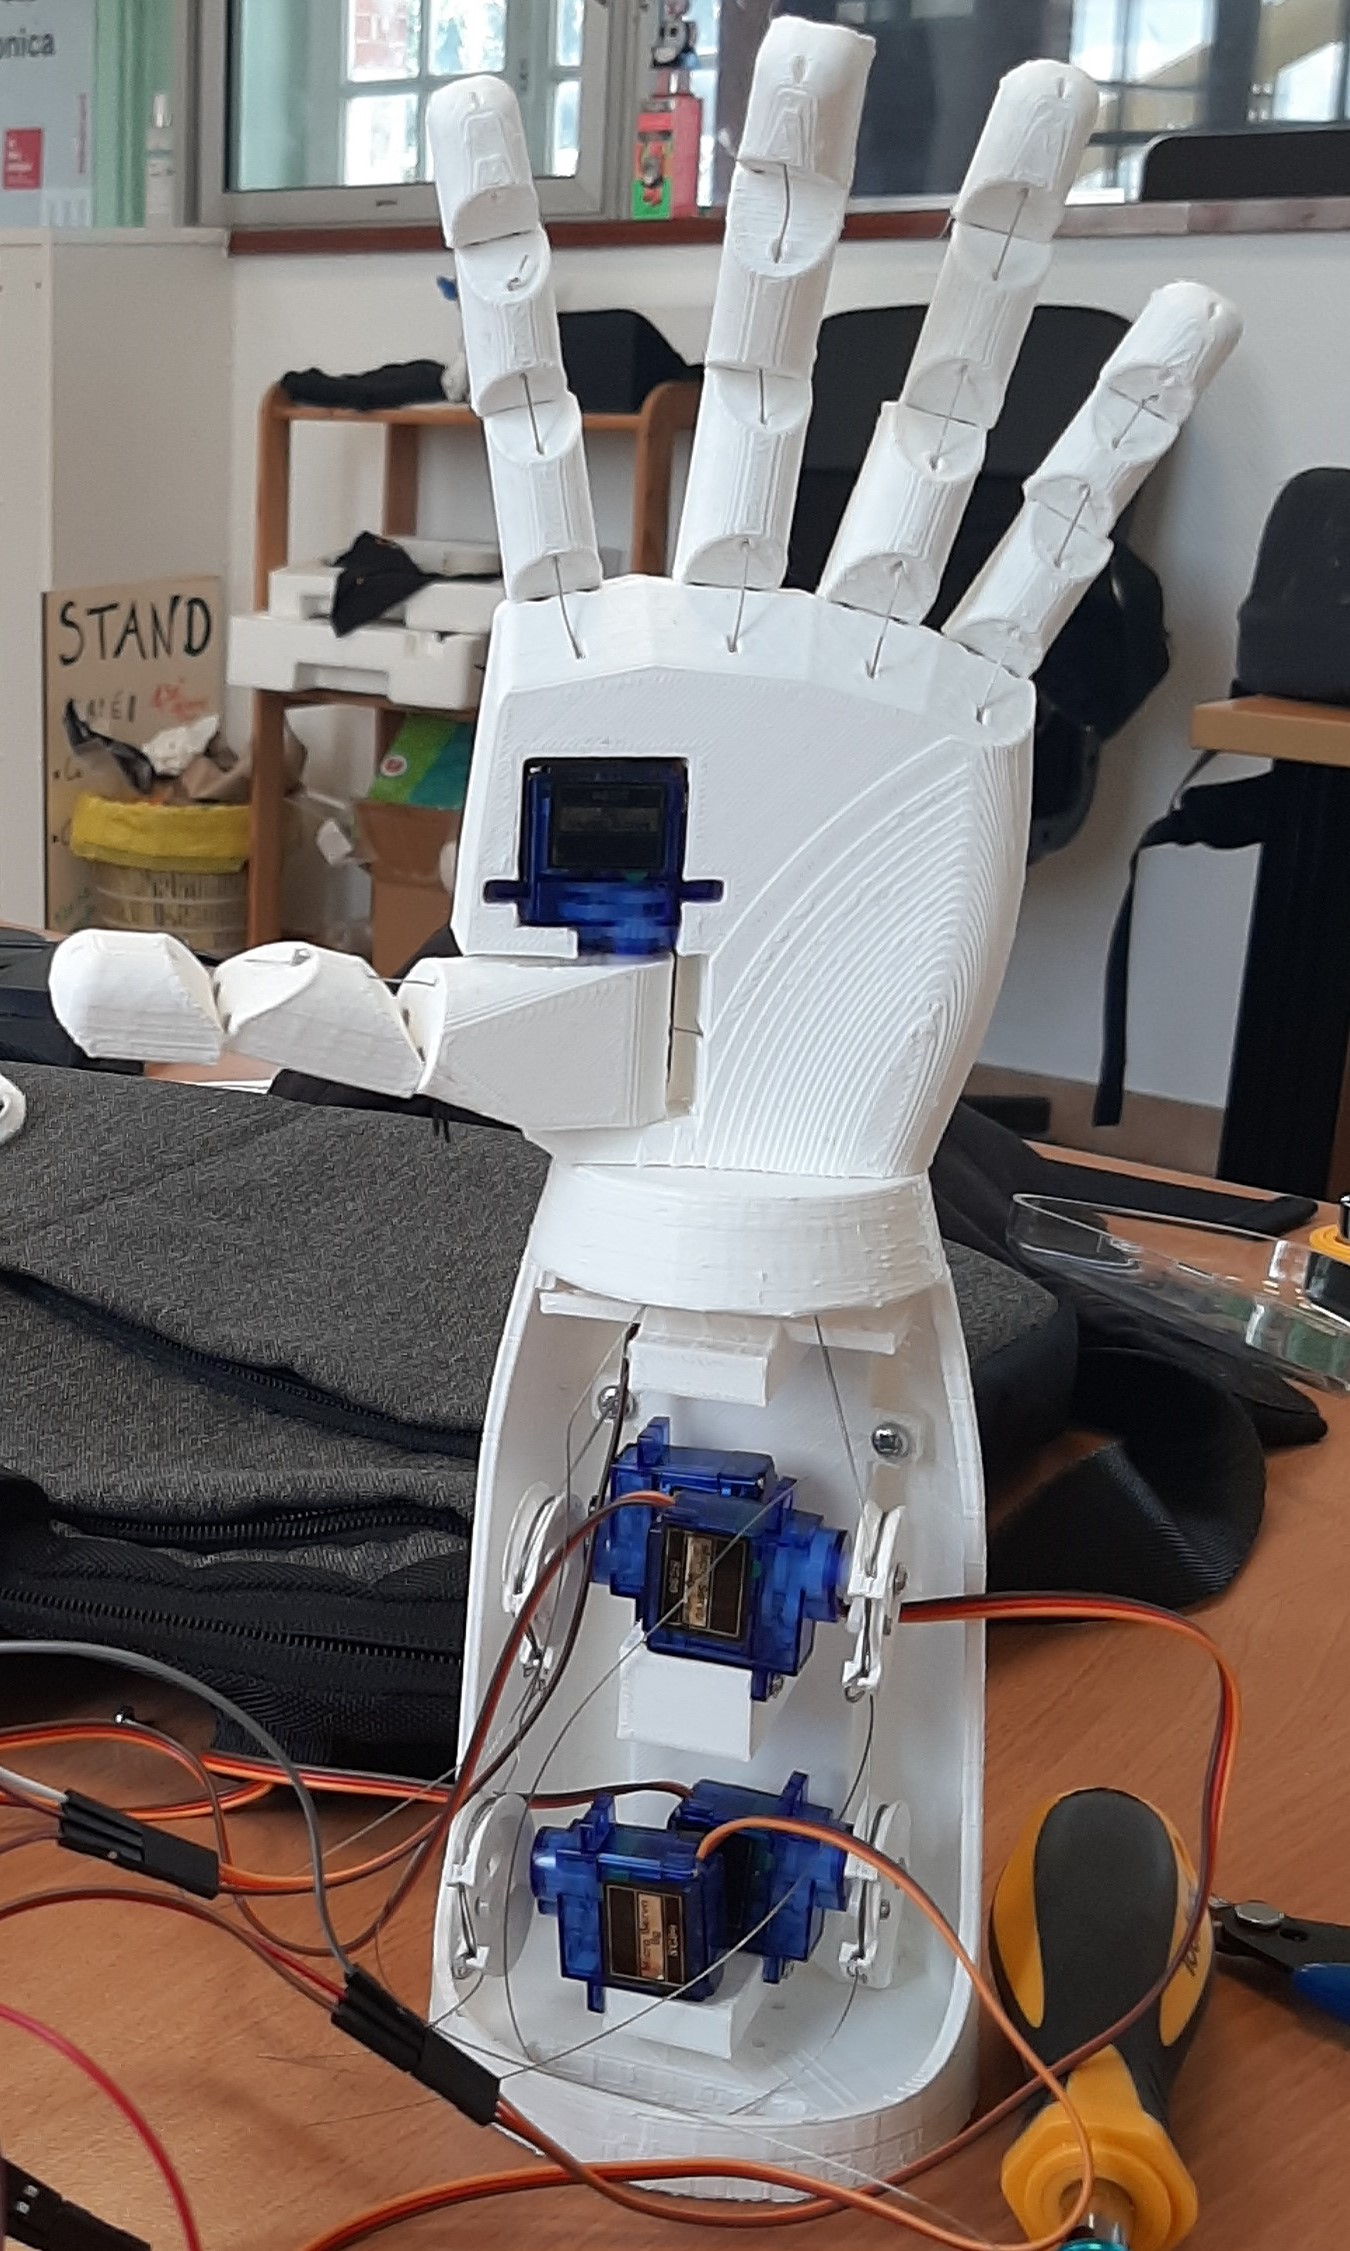
\includegraphics[width=200pt]{Déroulé/Jour_1/notre_version.jpg}
        \caption[Notre main]{Main robotique réalisée durant l'atelier}
        \label{fig:my_label}
    \end{figure}
\end{flushleft}

%provisoire
\newpage

\subsection{Où réaliser ses propres impressions 3D ?}

\begin{flushleft}
Vous n'avez pas d'imprimante 3D à la maison? Pas de problème !\vspace{0.2cm}

\textbf{À Nantes :}

\vspace{0.2cm}
\textbullet \, Contacter la société \href{https://dulse.fr/}{\textit{Dulse}}, membre du collectif \href{https://makeici.org/location-ateliers/nantes/}{\textit{Ici Nantes}} pour réaliser vos impressions. Le collectif propose également des formations certifiantes en impression 3D. (cliquer sur Ici Nantes pour avoir accès à leur catalogue de formations)\vspace{0.2cm}

\textbf{\large Note : }\textbf{\textit{\large Ces formations sont payantes mais sont éligibles au CPF (Compte Personnel de Formation).}}\vspace{0.2cm}

\textbullet \, Se rendre au FabLab de l'association \href{https://info.pingbase.net/faire-ensemble/#1598359300657-bc519d81-3b9f}{\textit{PiNG}}.\vspace{0.2cm}

\begin{multicols}{2}
    
\includegraphics[width=75pt,height=75pt]{Déroulé/Jour_1/Manuel d'utilisation/Images/6.jpg}
    
    \columnbreak
    
\textbf{Attention : }\textbf{\textit{Avant de pouvoir réaliser vos propres impressions sur les machines du FabLab, il vous faudra adhérer à PiNG. Renseignez vous sur leur site pour voir les offres proposées.}}\\
\end{multicols}
\end{flushleft}

\begin{flushleft}
\textbf{De manière un peu plus générale :}\\
\textbullet \vspace{2mm} Le \textit{pôle EMC2} a développé le site \href{https://meet3d.fr/imprimante/list}{\textit{Meet3D}}, qui recense les ressources en impression 3D.\vspace{0.2cm}

\textbullet \vspace{2mm} Il existe également une carte des FabLabs réalisée par le site \textit{Makery.info}.

\begin{figure}[!h]
    \centering
    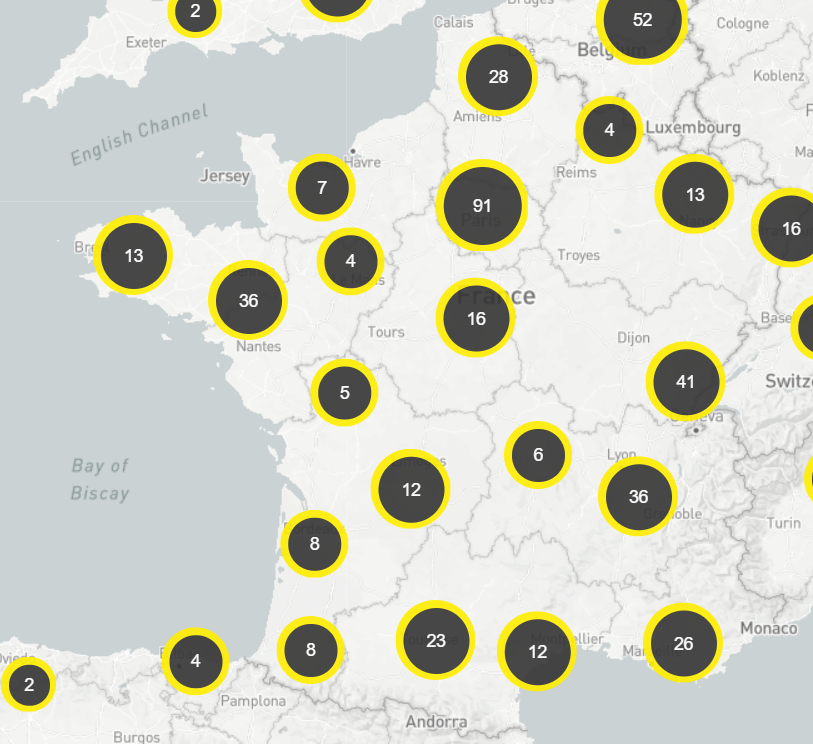
\includegraphics[width=250pt,height=250pt]{Déroulé/Jour_1/Carte_des_FabLab_France.PNG}
    \caption[Carte des FabLabs]{Carte de France des FabLabs}
    \label{fig:my_label}
\end{figure}
La carte détaillée avec les adresses est disponible \href{https://www.makery.info/labs-map/}{ici}.
\end{flushleft}

%provisoire
\newpage

\subsection{Utilisation de l'imprimante 3D}

\subsubsection{Notions de sécurité}

\begin{multicols}{2}


\includegraphics[width=50pt]{Déroulé/Jour_1/Manuel d'utilisation/Images/6.jpg}\\

\columnbreak
\begin{flushleft}
La buse et le plateau chauffent pendant l'utilisation. Attendre que l'imprimante ait refroidi avant d'essayer d'enlever les pièces ou les résidus de filaments.\\
\end{flushleft}

\end{multicols}

\begin{multicols}{2}


\includegraphics[]{Déroulé/Jour_1/Manuel d'utilisation/Images/1.PNG}\\

\columnbreak
\begin{flushleft}
L’imprimante présente des parties mobiles pouvant être dangereuses.
Ne pas toucher la machine pendant son fonctionnement.\\
\end{flushleft}

\end{multicols}

\begin{multicols}{2}


\includegraphics[]{Déroulé/Jour_1/Manuel d'utilisation/Images/5.PNG}\\

\columnbreak
\begin{flushleft}
Ne pas laisser l'imprimante à la portée des enfants.
\end{flushleft}

\end{multicols}

\begin{multicols}{2}

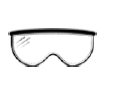
\includegraphics[]{Déroulé/Jour_1/Manuel d'utilisation/Images/2.PNG}\\

\columnbreak
\begin{flushleft}
Il est recommmandé d'utiliser des lunettes de protection lorsque l'on nettoie les pièces pour éviter que des projections entre en contact avec les yeux.\\
\end{flushleft}

\end{multicols}

\begin{multicols}{2}


\includegraphics[]{Déroulé/Jour_1/Manuel d'utilisation/Images/3.PNG}\\

\columnbreak
\begin{flushleft}
Ne pas rester trop proche de l'imprimante pendant l'impression, les vapeurs peuvent être dangereuses. Utiliser si possible l'imprimante dans une pièce aérée ou ventilée.
\end{flushleft}

\end{multicols}

\begin{multicols}{2}


\includegraphics[]{Déroulé/Jour_1/Manuel d'utilisation/Images/4.PNG}\\

\columnbreak
\begin{flushleft}
Ne pas mettre d'eau sur l'imprimante.
\end{flushleft}

\end{multicols}

%provisoire
\newpage

\subsubsection{Prise en main du logiciel \textit{Ultimaker Cura}}

\begin{flushleft}
\textbf{Installation du logiciel :}\vskip0.4cm

\textbullet \, Se rendre sur le site : \url{https://ultimaker.com/fr/software/ultimaker-cura}\vspace{0.2cm}

\textbullet \vspace{2mm} Aller dans la section \textit{Logiciel} :
\begin{figure}[!h]
    \centering
    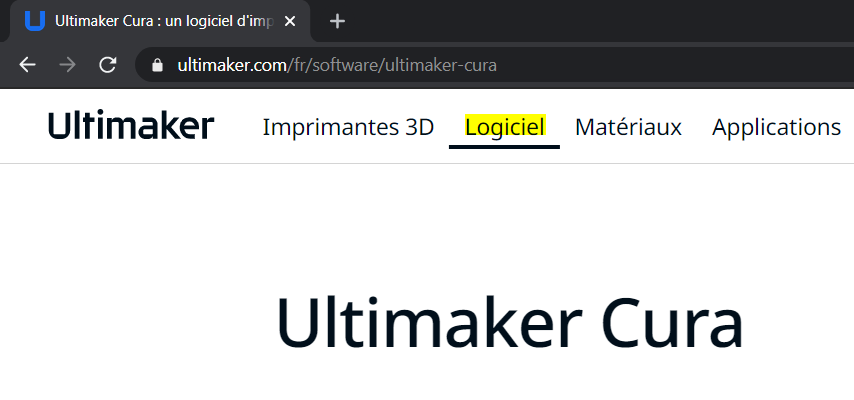
\includegraphics[width=400pt]{Déroulé/Jour_1/étape1.PNG}
    \caption{Installation Cura - \'Etape 1}
    \label{fig:my_label}
\end{figure}

\textbullet \, Descendre jusqu'à \textit{Ultimaker Cura} et cliquer sur \textit{En savoir plus} :
\begin{figure}[!h]
    \centering
    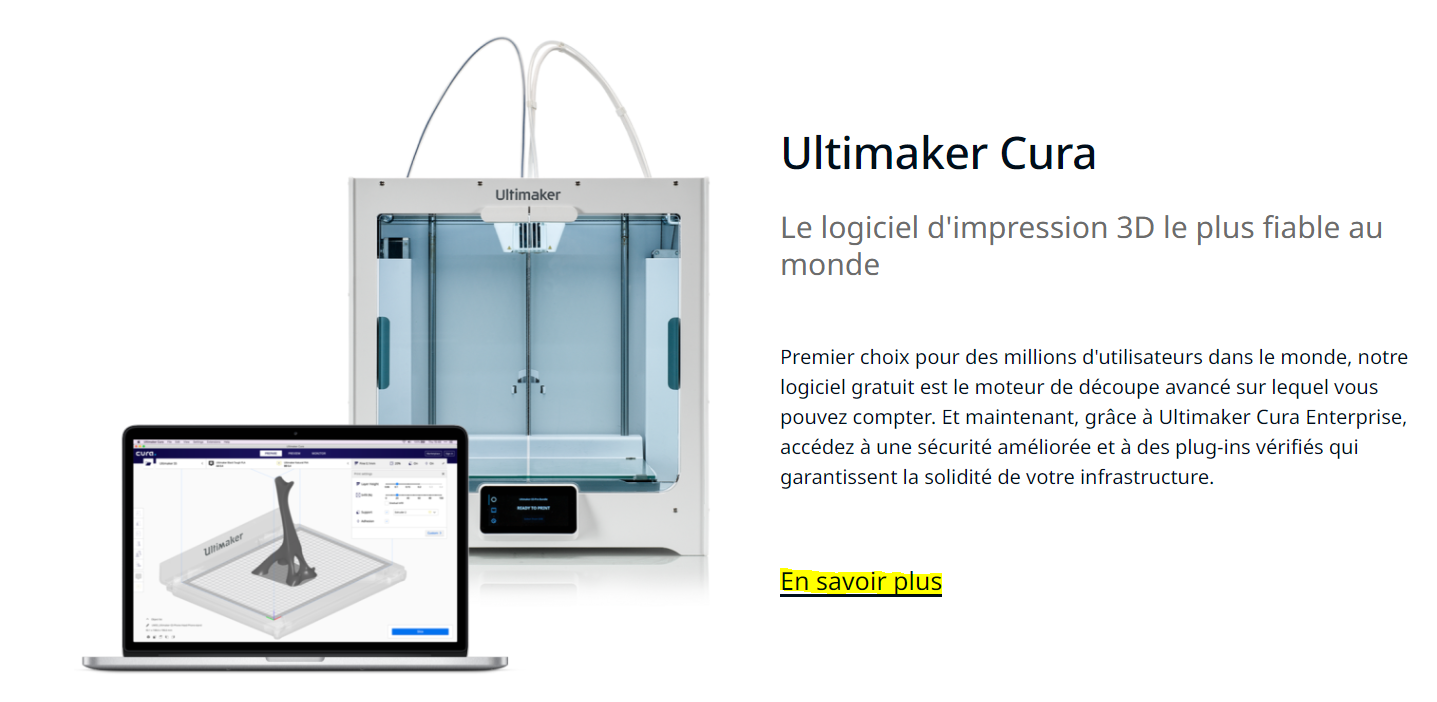
\includegraphics[width=400pt]{Déroulé/Jour_1/étape2.PNG}
    \caption[\'Etape 2]{Installation Cura - \'Etape 2}
    \label{fig:my_label}
\end{figure}

%provisoire
\newpage

\textbullet \, Cliquer sur \textit{Télécharger gratuitement} :
\begin{figure}[!h]
    \centering
    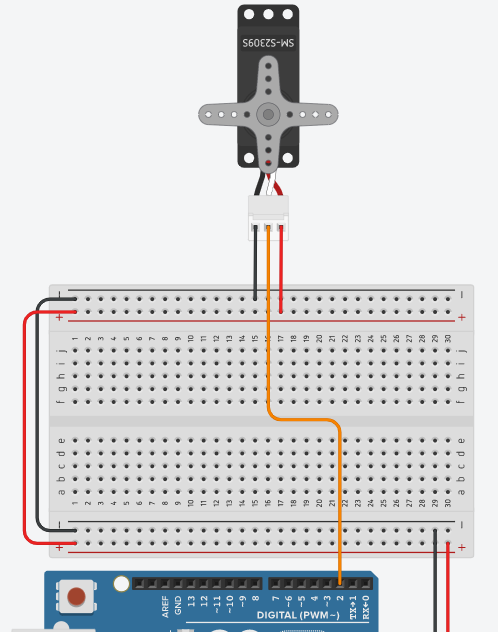
\includegraphics[width=300pt]{Déroulé/Jour_1/étape3.PNG}
    \caption[\'Etape 3]{Installation Cura - \'Etape 3}
    \label{fig:my_label}
\end{figure}
\end{flushleft}

\begin{flushleft}
\textbf{Configuration du logiciel :}\vspace{0.4cm}

\textbullet \, Cliquer sur la petite flèche :
\begin{figure}[!h]
    \centering
    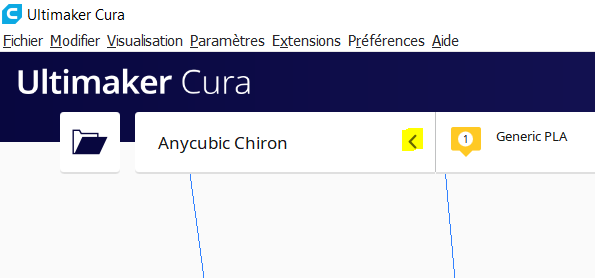
\includegraphics[width=300pt]{Déroulé/Jour_1/réglagesCura_étape1.PNG}
    \caption{Configuration Cura - \'Etape 1}
    \label{fig:my_label}
\end{figure}

%provisoire
\newpage

\textbullet \, Cliquer sur \textit{ajouter une imprimante} :
\begin{figure}[!h]
    \centering
    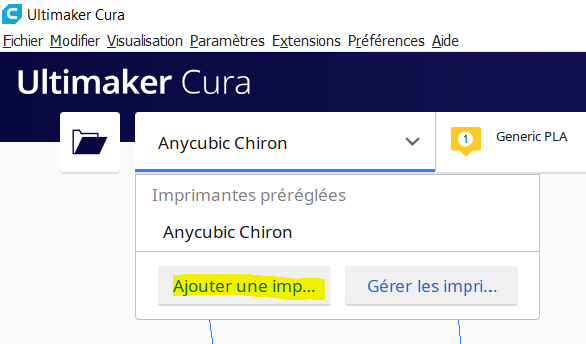
\includegraphics[width=300pt]{Déroulé/Jour_1/réglagesCura_étape2.PNG}
    \caption[\'Etape 2]{Configuration Cura - \'Etape 2}
    \label{fig:my_label}
\end{figure}

\textbullet \, Choisir son imprimante en réseau si elle est disponible, ou la sélectionner manuellement en allant dans \textit{hors réseau} sinon, puis l'ajouter :
\begin{figure}[!h]
    \centering
    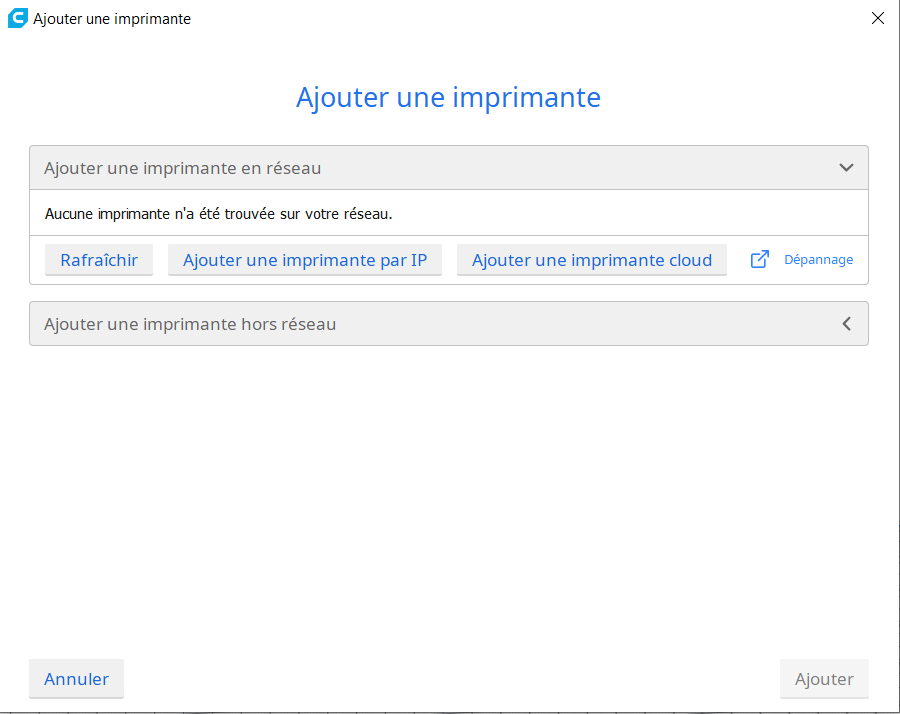
\includegraphics[width=300pt]{Déroulé/Jour_1/réglagesCura_étape3.PNG}
    \caption[\'Etape 3]{Configuration Cura - \'Etape 3}
    \label{fig:my_label}
\end{figure}

%provisoire
\newpage

\textbullet \, Cliquer sur la petite flèche pour choisir le type de filament que vous allez utiliser :
\begin{figure}[!h]
    \centering
    
\includegraphics[width=300pt]{Déroulé/Jour_1/réglagesCura_étape4.PNG}
    \caption[\'Etape 4]{Configuration Cura - \'Etape 4}
    \label{fig:my_label}
\end{figure}

\textbullet \, Cliquer sur le petit crayon pour régler les paramètres d'impression :
\begin{figure}[!h]
    \centering
    
\includegraphics[width=300pt]{Déroulé/Jour_1/réglagesCura_étape5.PNG}
    \caption[\'Etape 5]{Configuration Cura - \'Etape 5}
    \label{fig:my_label}
\end{figure}

\textbullet \, Modifier les paramètres d'impression comme suit :\\
\begin{figure}[!h]
    \centering
    \begin{tabular}{|l|l|l|}
    
    \hline Catégorie & Nom du paramètre & Valeur\\
    \hline Qualité & Hauteur de la couche & 0.3 mm\\
    \hline Coque & \'Epaisseur de la paroi & 0.5 mm\\
    \hline & Nombre de lignes de la paroi & 1\\
    \hline & \'Epaisseur du dessus/dessous & 0.8 mm\\
    \hline & \'Epaisseur du dessus & 0.8 mm\\
    \hline & Couche supérieure & 3\\
    \hline & \'Epaisseur du dessous & 0.8 mm\\
    \hline & Couche inférieure & 3\\
    \hline & Expansion horizontale & 0 mm\\
    \hline Remplissage & Densité du remplissage & 17.5\% \\
    \hline & Motif de remplissage & Grille\\
    \hline Matériau & Température d'impression & 200°C\\
    \hline & Température du plateau & 85°C\\
    \hline Vitesse & Vitesse d'impression & 80mm/s\\
    \hline Déplacement & Activer la rétraction & Oui\\
    \hline Refroidissement & Activer le refroidissement de l'impression & Oui\\
    \hline & Vitesse du ventilateur & 100\% \\
    \hline Supports & Générer les supports & Non \\
    \hline Adhérence du plateau & Type d'adhérence du plateau & Bordure \\
    \hline 
    
    \end{tabular}
    \caption[\'Etape 6]{Configuration Cura - \'Etape 6}
    \label{fig:my_label}
\end{figure}

\begin{multicols}{2}
    
\includegraphics[width=60pt,height=60pt]{Déroulé/Jour_1/Manuel d'utilisation/Images/6.jpg}
    
    \columnbreak
    
\textbf{\large Attention : }\textbf{\textit{L'imprimante que nous avons utilisé pour le projet est une Chiron de chez Anycubic, et le type filament utilisé est le PLA. Les paramètres d'impression seront peut-être à régler différemment si vous utilisez une autre imprimante et un autre type de filament.}}\\\vspace{0.2cm}
\end{multicols}

\textbullet \, Aller dans \textit{fichier} puis \textit{Ouvrir le(s) fichier(s)} et sélectionner celui que vous voulez imprimer :
\begin{figure}[!h]
    \centering
    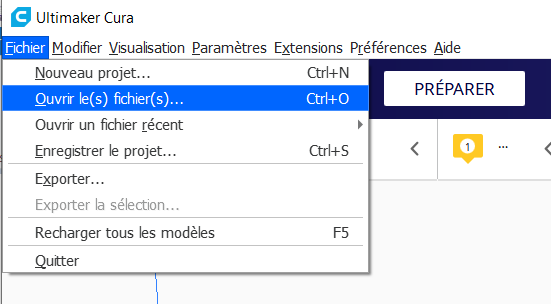
\includegraphics[width=300pt]{Déroulé/Jour_1/réglagesCura_étape7.PNG}
    \caption[\'Etape 7]{Configuration Cura - \'Etape 7}
    \label{fig:my_label}
\end{figure}


\includegraphics[width=30pt,height=30pt]{Déroulé/Jour_1/idée.png}
\textbf{\large Astuce : }\textbf{\textit{\large Si le plateau de votre imprimante est assez grand, il est possible d'imprimer plusieurs pièces simultanément. Pour cela il faut les positionner de part et d'autre du plateau virtuel sur Cura. Pour ce faire, cliquez sur la pièce que vous voulez déplacer et bouger la en restant appuyé sur la flèche correspondant à la direction souhaitée.}}\\\vspace{0.2cm}


\includegraphics[width=30pt,height=30pt]{Déroulé/Jour_1/idée.png}
\textbf{\large Astuce : }\textbf{\textit{\large La température de la pièce dans laquelle vous êtes influe également sur la qualité de votre impression.}}\\
\end{flushleft}

\newpage

%---------------------------------------------------------------------------------------------------------------------------------------------------%

\section{Introduction à l'électronique}
\subsection{Définition de quelques termes}
\begin{flushleft}
    Avant toute chose, nous allons définir assez simplement quelques termes concernant le matériel que nous allons utiliser:\\\vskip0.4cm
    Servomoteur : Sa fonction principale est d'assurer la reproduction d'un mouvement en réponse à une commande externe. En l'occurence la commande sera envoyée par nos potentiomètres linéaires.\\
    
    \begin{multicols}{2}
    
\includegraphics[width=60pt,height=60pt]{Déroulé/Jour_1/Manuel d'utilisation/Images/6.jpg}
    
    \columnbreak
    
    \textbf{\large Attention : }\textbf{\textit{ Les servomoteurs que nous utilisons ici sont des servomoteurs standards et ont une plage de mouvement entre 0° et 180°.}}\\\vspace{0.2cm}
    \end{multicols}

    Potentiomètre linéaire : Un potentiomètre linéaire est une résistance variable permettant d'ajuster la valeur de certains paramètres. En l'occurence le paramètre ajusté sera la position angulaire du servomoteur correspondant.\\\vspace{0.2cm}
    
    Câbles Dupont mâle-mâle : Ces câbles permettent de créer une connexion sur une platine d'essai sans avoir à réaliser de soudure. Ils sont dits "mâles-mâles" car ils présentent de chaque côté une petite pointe venant s'insérer dans les ports de connexions.\\\vspace{0.2cm}
    
    Platine d'essai (Breadboard en anglais) : Dispositif permettant de réaliser le prototypage et le test d'un circuit électronique sans avoir à réaliser de soudure.\\\vspace{0.2cm}
    
    Entrée digitale : \'Egalement appelée entrée numérique. Ce sont des entrées ne pouvant prendre que 2 valeurs : 0 (le système est à l'arrêt) et 1 (le système est en fonctionnement).\\\vspace{0.2cm}
    
    Entrée analogique : Elle s'oppose à l'entrée digitale et permet de recueillir un signal électrique variable sur une plage de valeur définie au préalable.
\end{flushleft}

\subsection{Ce que l'on utilise pour cet atelier }
\begin{flushleft}
    Pour programmer le mouvement de cette main, nous allons utiliser le matériel suivant :\\
    \begin{figure}[!h]
        \centering
        \begin{tabular}{|l|l|}
            \hline Type & Quantité/unité\\
            \hline Carte Arduino Uno & 1\\
            \hline Câbles Dupont mâle-mâle & 32\\
            \hline Potentiomètres linéaires 10k$\Omega$ & 5\\
            \hline Servomoteurs 9g SG-90 & 5\\
            \hline Platine d'essai & 1\\
            \hline Pile 9V & 1\\
            \hline Support de pile (banchement sur port secteur) & 1\\
            \hline
        \end{tabular}
        \caption[Matériel électronique]{Liste du matériel électronique nécessaire}
        \label{2.1}
    \end{figure}
\end{flushleft}

%provisoire
\newpage

\subsection{Fonctionnement des composants}

\begin{flushleft}
    \textbf{La platine d'essai :}\vspace{0.4cm}
    \begin{figure}[!h]
        \centering
        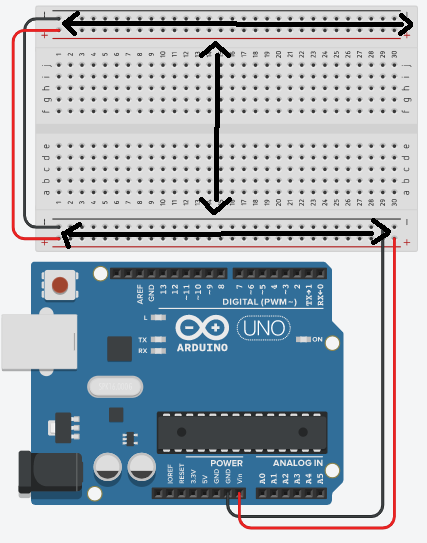
\includegraphics[height=300pt]{Déroulé/Jour_2/breadboard.PNG}
        \caption[Platine d'essai]{Sens des connexions sur la platine d'essai}
        \label{2.2}
    \end{figure}

    \textbf{La carte Arduino :}\vspace{0.4cm}
    \begin{figure}[!h]
        \centering
        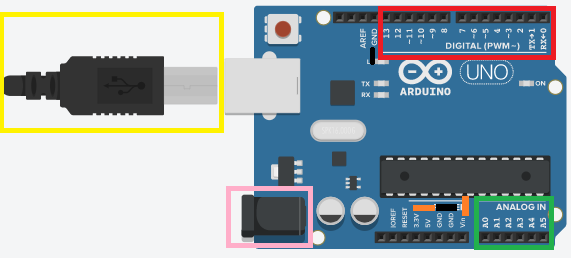
\includegraphics[width=300pt]{Déroulé/Jour_2/Carte.PNG}
        \caption[Carte Arduino]{Description des différents ports de la carte Arduino}
        \label{fig:my_label}
    \end{figure}
    \end{flushleft}
    
    %provisoire
    \newpage
    
    \begin{flushleft}
    \underline{\textit{\large Légende :}}\vspace{0.4cm}

    \begin{itemize}
        \item \begin{flushleft}\textcolor{orange}{Traits orange :} Ce sont les ports de la carte permettant d'alimenter en tension la platine d'essai. Cette carte présente une alimentation en 3.3V, une en 5V et celle qui va nous intéresser étant donné que nous allons alimenter l'Arduino avec une pile 9V : $V_{in}$.\vspace{0.2cm}
        \end{flushleft}
        \begin{flushleft}
        \begin{multicols}{2}
        
\includegraphics[width=60pt,height=60pt]{Déroulé/Jour_1/Manuel d'utilisation/Images/6.jpg}
    
        \columnbreak
    
        \textbf{\large Attention : }\textbf{\textit{ La carte Arduino Uno peut supporter une tension d'alimentation externe entre 6V et 20V mais il est recommandé que cette tension soit comprise entre 7V et 12V.}}\\\vspace{0.2cm}
        \end{multicols}
        \end{flushleft}
        
        \item \textcolor{black}{Traits noir :} Ce sont les ports de la carte permettant de mettre les différents composants branchés à la masse (= gnd sur la carte $\Leftrightarrow$ ground en anglais). Cela correspond à une tension de 0V.\vspace{0.2cm}
        
        
\includegraphics[width=30pt,height=30pt]{Déroulé/Jour_1/idée.png}
        \textbf{\large Astuce : }\textbf{\textit{\large En pratique, lorsque l'on utilise une platine d'essai, on connecte un des ports de masse de l'Arduino à la ligne de masse de la platine d'essai avec un câble Dupont (Voir figure 15).}}\\\vspace{0.2cm}
        
        \item \textcolor{yellow}{Carré jaune :} C'est le port d'alimentation en USB de la carte Arduino. Il permet de téléverser le programme de l'ordinateur sur le microprocesseur de la carte, et également de l'alimenter si on le laisser branché une fois le programme téléversé.\\\vspace{0.2cm}
        
        \item \textcolor{pink}{Carré rose :} C'est le port d'alimentation sur secteur de l'Arduino. C'est celui qui va nous permettre d'alimenter la carte lors de notre projet.\\\vspace{0.2cm}
        
        \item \textcolor{green}{Carré vert :} Ce sont les ports d'entrées analogiques de la carte. Ici ils vont nous servir à brancher les différents potentiomètres.\\\vspace{0.2cm}
        
        \item \textcolor{red}{Carré rouge :} Ce sont les ports d'entrées digitales de la carte. Ici ils vont nous servir à brancher les différents servomoteurs.\vspace{0.2cm}
    \end{itemize}
    
    %provisoire
    \newpage
    
    \textbf{Les potentiomètres :}\vspace{0.4cm}
    \begin{figure}[!h]
        \centering
        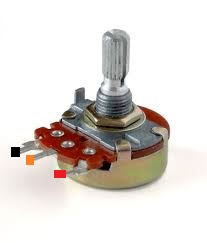
\includegraphics[]{Déroulé/Jour_2/potentiomètre.jpg}
        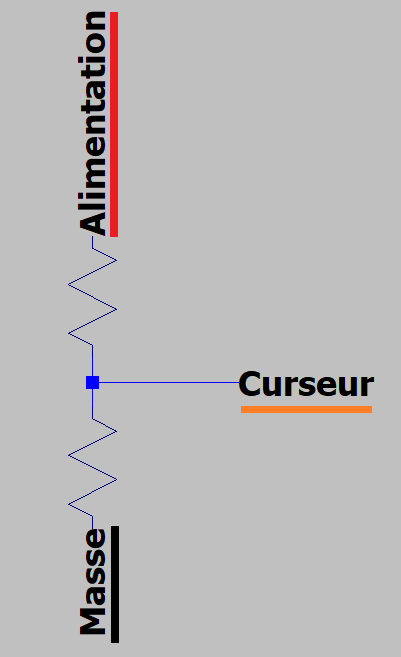
\includegraphics[width=100pt]{Déroulé/Jour_2/schéma_potentiomètre.PNG}
        \caption[Potentiomètre]{Photo et schéma électronique d'un potentiomètre linéaire}
        \label{2.4}
    \end{figure}
    \begin{flushleft}
    \underline{\textit{\large Légende :}}\vspace{0.4cm}
    
        \begin{itemize}
    \item \textcolor{black}{Point et trait noir :} Port relié à la masse de la platine d'essai.\vspace{0.2cm}
    \item \textcolor{red}{Point et trait rouge :} Port relié à l'alimentation de la platine d'essai.\vspace{0.2cm}
    \item \textcolor{orange}{Point et trait orange :} Port relié au curseur du potentiomètre et à l'entrée analogique de l'Arduino, permettant de lire la valeur du potentiomètre.
    \end{itemize}
    \end{flushleft}
    
    Dans notre cas, faire bouger le curseur du potentiomètre va permettre d'envoyer une certaine valeur de tension au servomoteur en la convertissant en une position angulaire (entre 0° et 180°). Cette position sera alors lue par le servomoteur qui bougera jusqu'à atteindre la position demandée.\\
    \end{flushleft}
    
    \begin{flushleft}
    \textbf{Le servomoteur SG-90 :}\vspace{0.4cm}
    \end{flushleft}
    \begin{figure}[!h]
        \centering
        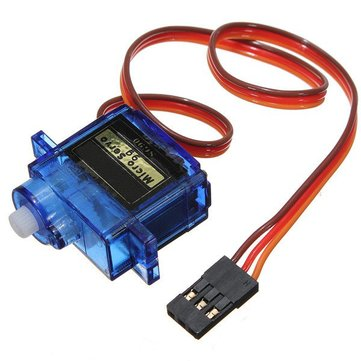
\includegraphics[width=150pt,height=150pt]{Déroulé/Jour_2/SG90.jpg}
        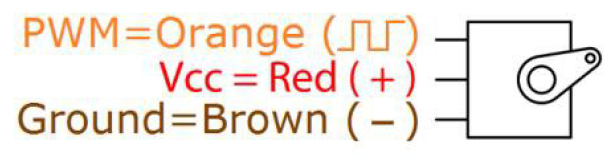
\includegraphics[width=300pt]{Déroulé/Jour_2/schéma_SG90.PNG}
        \caption[Servomoteur SG-90]{Photo et schéma du servomoteur utilisé}
        \label{2.5}
    \end{figure}
    
    \begin{flushleft}
    \textbf{\large Note : }\textbf{\textit{ PWM (= Pulse With Modulation en anglais) correspond à une entrée digitale sur l'Arduino.}}\\\vspace{0.2cm}
    \end{flushleft}
    
    %provisoire
    \newpage
    
    \begin{flushleft}
    \textbf{La pile :}\vspace{0.4cm}
    \end{flushleft}
    \begin{figure}[!h]
        \centering
        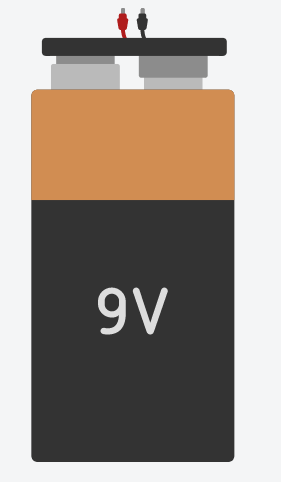
\includegraphics[height=200pt]{Déroulé/Jour_2/pile.PNG}
        \caption[Pile]{Schéma de la pile 9V}
        \label{fig:my_label}
    \end{figure}
    \begin{flushleft}
    \underline{\textit{\large Légende :}}\vspace{0.4cm}
    
    \begin{itemize}
    \item \textcolor{red}{Câble rouge :} Câble d'alimentation 9V de la pile (borne +).\vspace{0.2cm}
    \item \textcolor{black}{Câble noir :} Câble de masse de la pile (borne -).
    \end{itemize}
    \end{flushleft}
    
\subsection{Où acheter son matériel ?}

\begin{flushleft}
     Il est très facile de vous procurer le matériel. Il y a énormément de sites et/ou magasins spécialisés dans la vente de composants électroniques pour les particuliers. Un grand nombre de composants sont également disponibles sur des sites comme Amazon, Ebay, etc..
\end{flushleft}


%---------------------------------------------------------------------------------------------------------------------------------------------------%

%provisoire
\newpage

\section{Réalisation de la main}


\subsection{Montage de la main}

\begin{flushleft}
\begin{figure}[!h]
    \centering
\begin{tabular}{|l|l|}
    \hline objet & quantité nécessaire  \\
    \hline câble élastique pour les articulations & 45cm/doigt\\
    \hline câble métal pour doigts & 54cm/doigt\\
    \hline super glue ou pistolet à colle chaude & environ 1 tube\\
    \hline vis & 14 (utiliser celles fournies avec les servomoteurs)\\
    \hline
\end{tabular}
\caption{Liste du matériel nécessaire au montage}
\label{fig:my_label}
\end{figure}
\end{flushleft}

\begin{flushleft}
\textbullet \, Positionner les différentes phalanges autour de la paume pour visualiser le résultat final :
\end{flushleft}

\begin{figure}[!h]
    \centering
    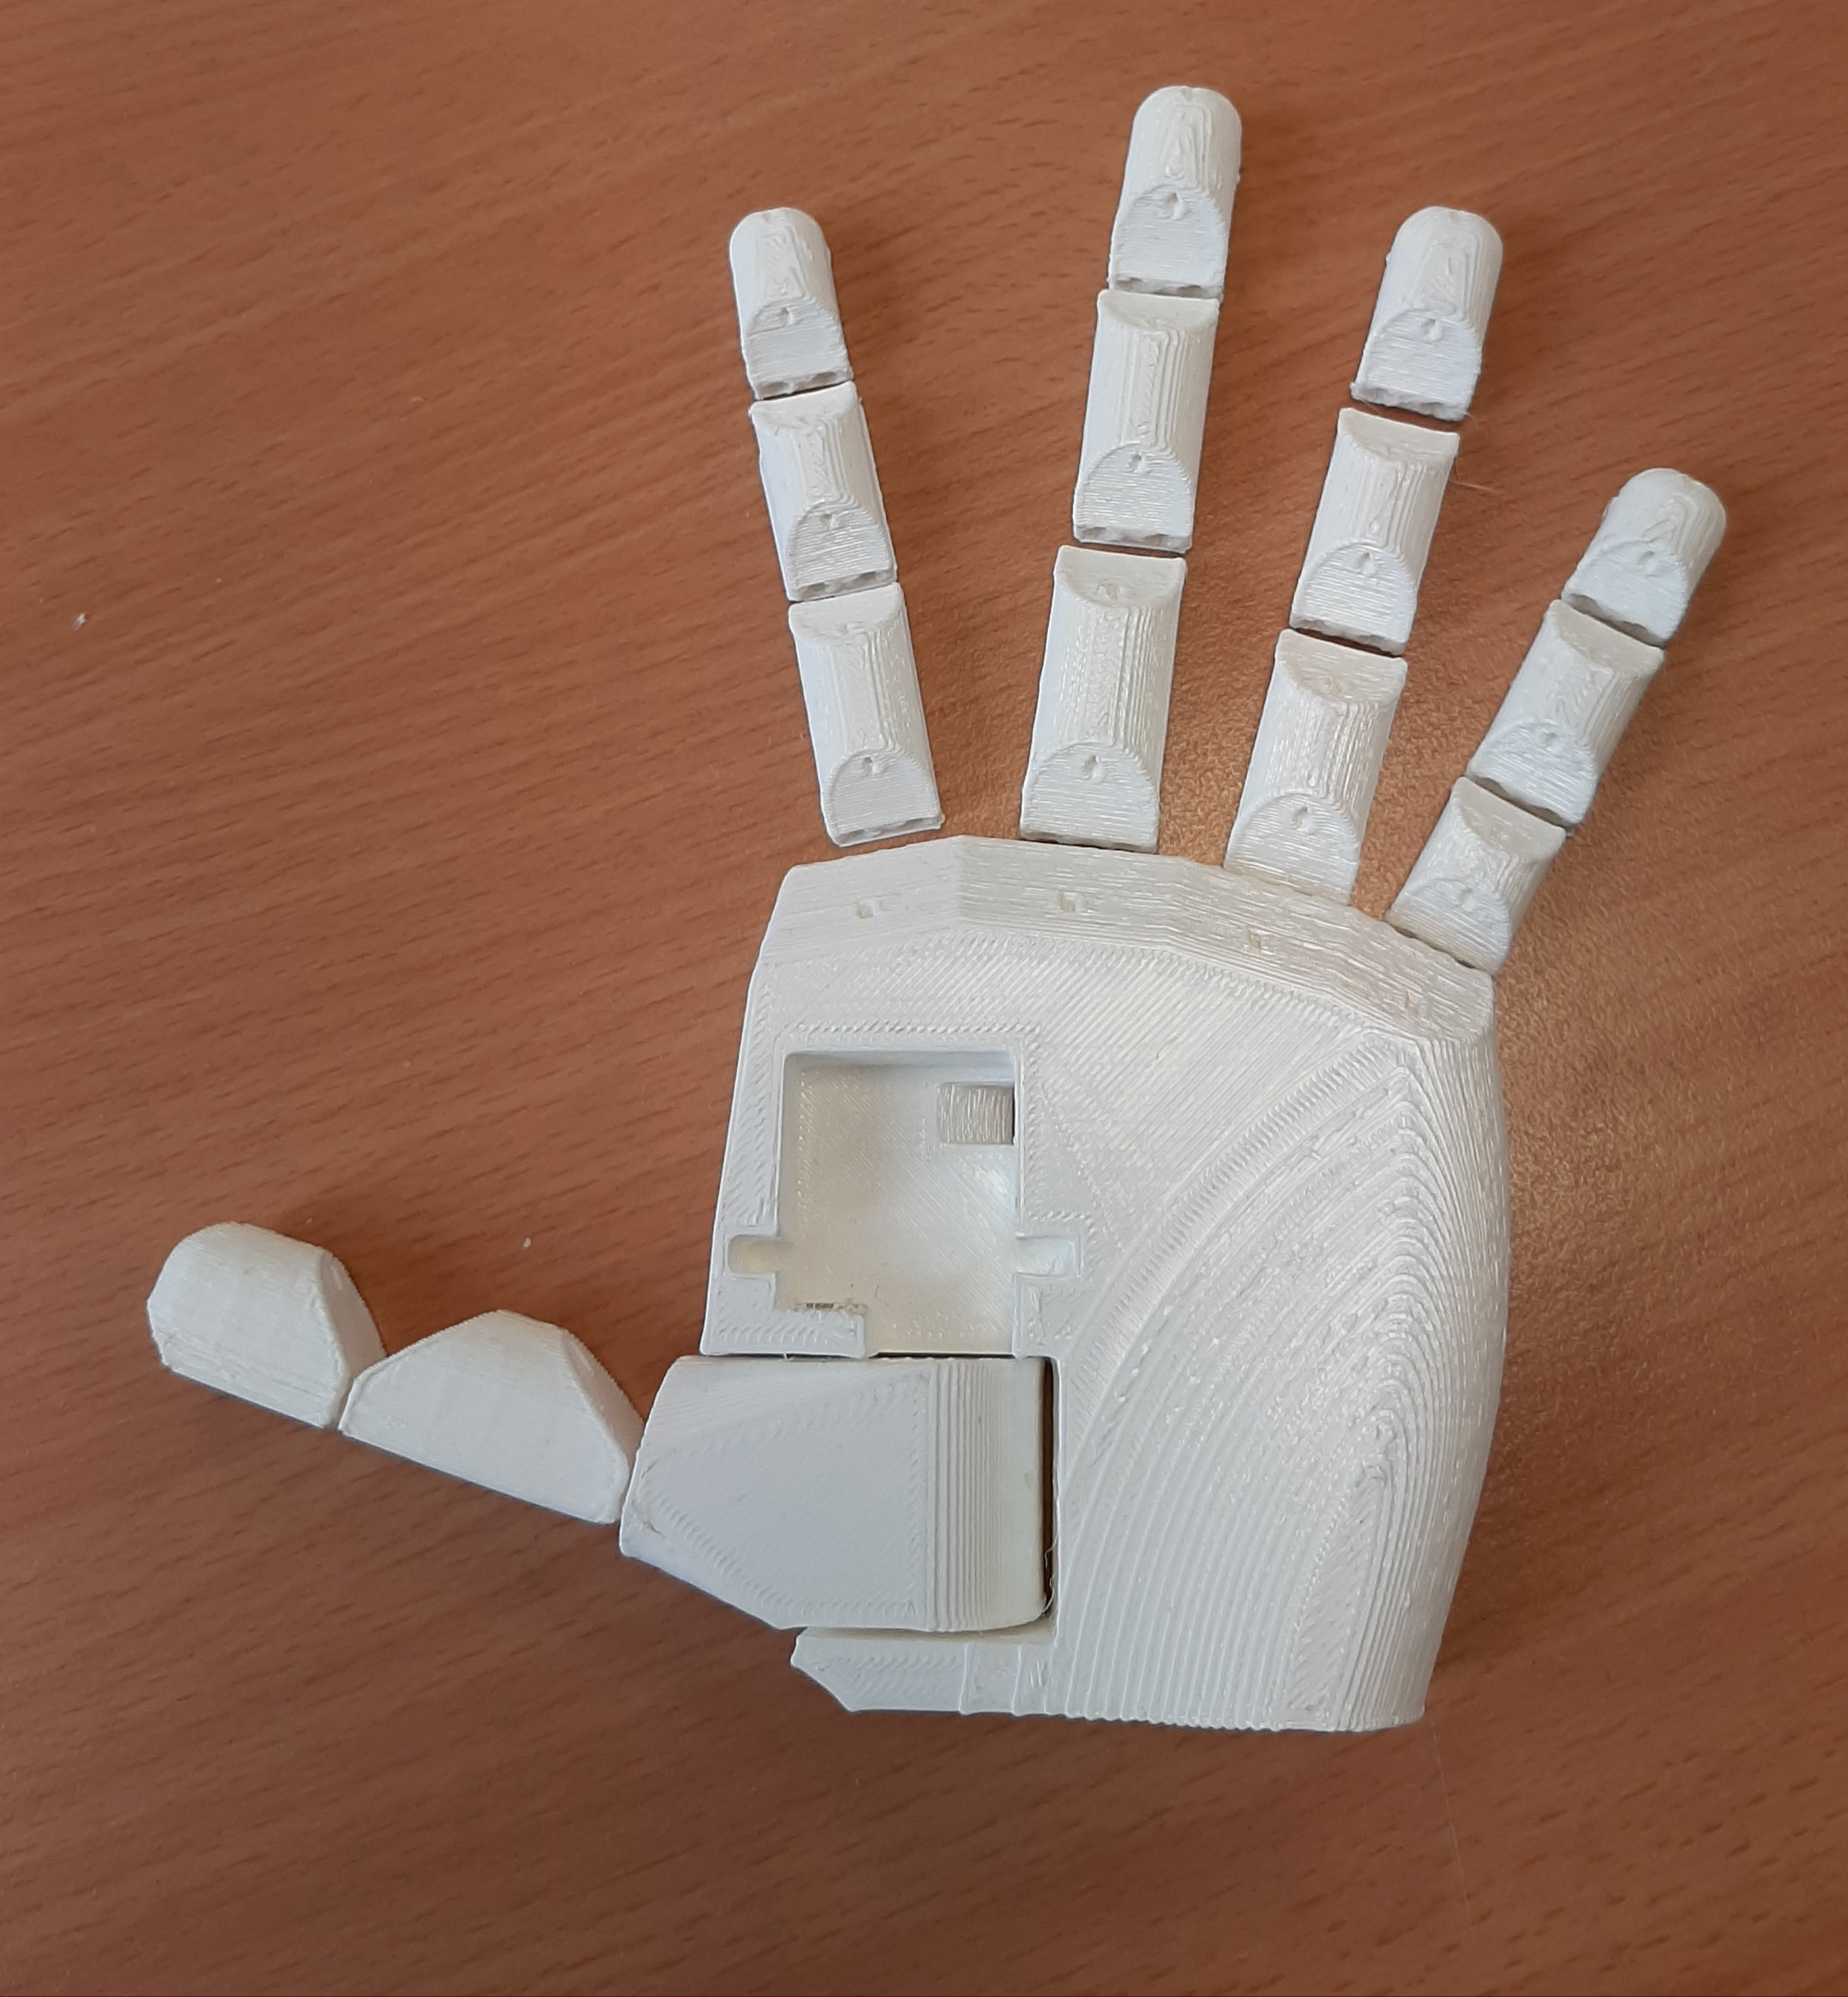
\includegraphics[width=400pt,height=400pt]{Déroulé/Jour_3/Montage de la main/étape 1.jpg}
    \caption{Montage de la main - \'Etape 1}
    \label{fig:my_label}
\end{figure}

%provisoire
\newpage

\begin{flushleft}
\textbullet \, Passer le câble souple une 1ère fois dans les différentes articulations des doigts puis dans la paume, et faire un 2ème tour si nécessaire pour que le fil soit plus tendu :
\end{flushleft}

\begin{figure}[!h]
    \centering
    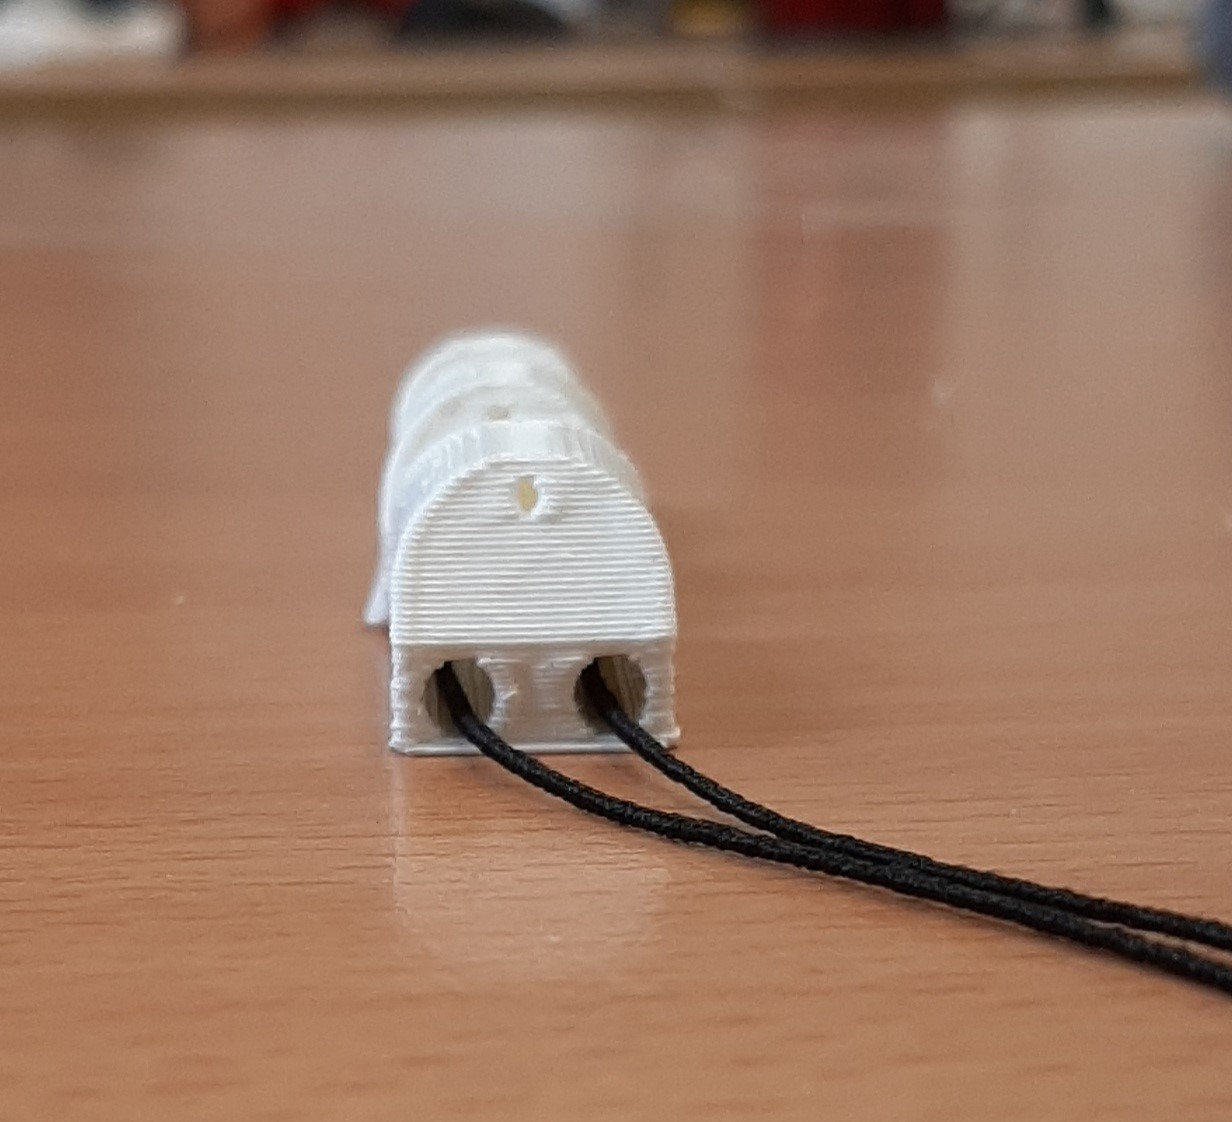
\includegraphics[width=200pt, height=200pt]{Déroulé/Jour_3/Montage de la main/étape2_1.jpg}
    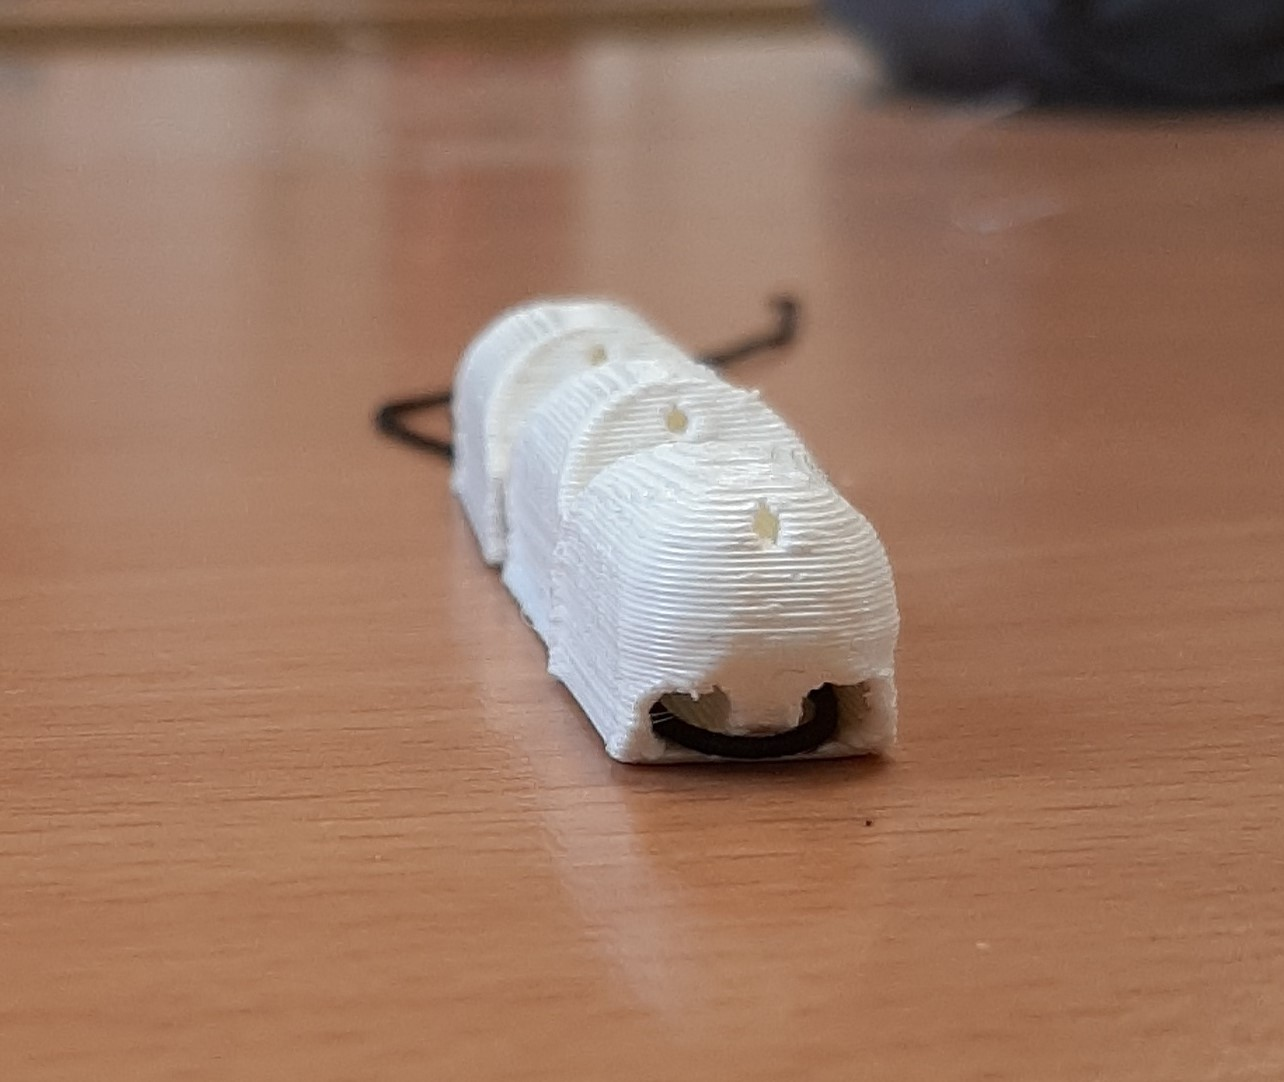
\includegraphics[width=200pt, height=200pt]{Déroulé/Jour_3/Montage de la main/étape2_2.jpg}
    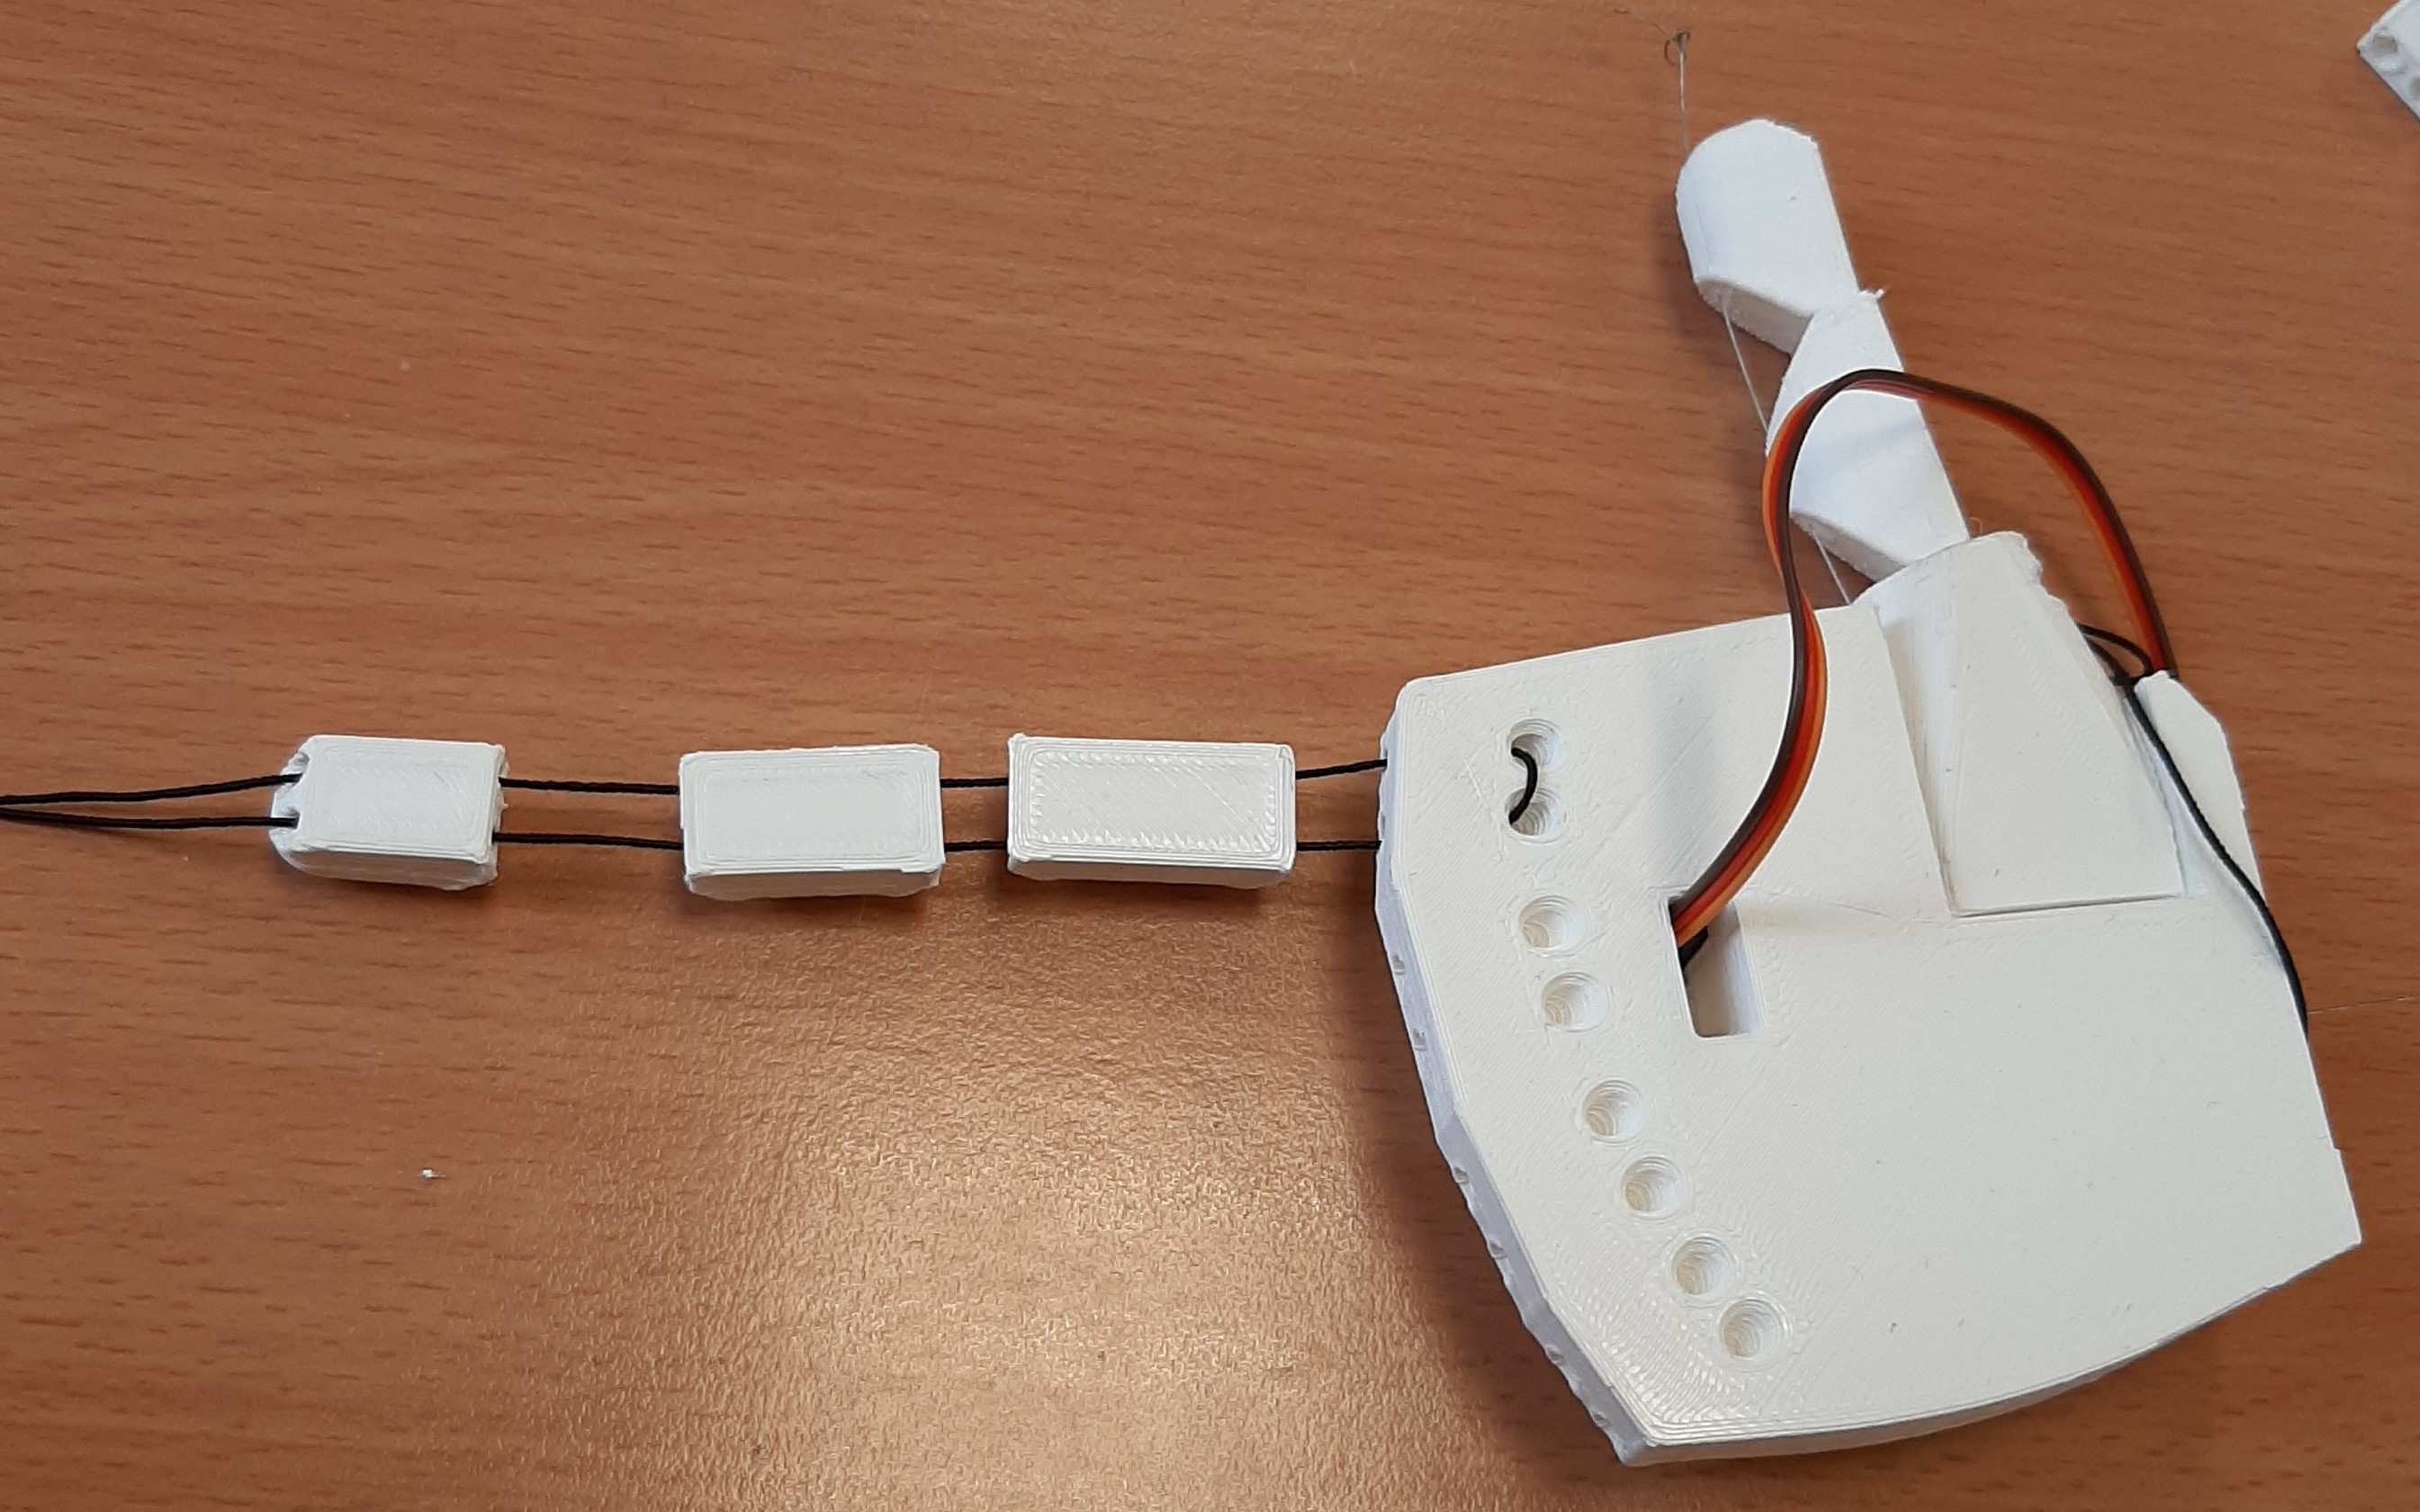
\includegraphics[width=250pt, height=200pt]{Déroulé/Jour_3/Montage de la main/étape2_3.jpg}
    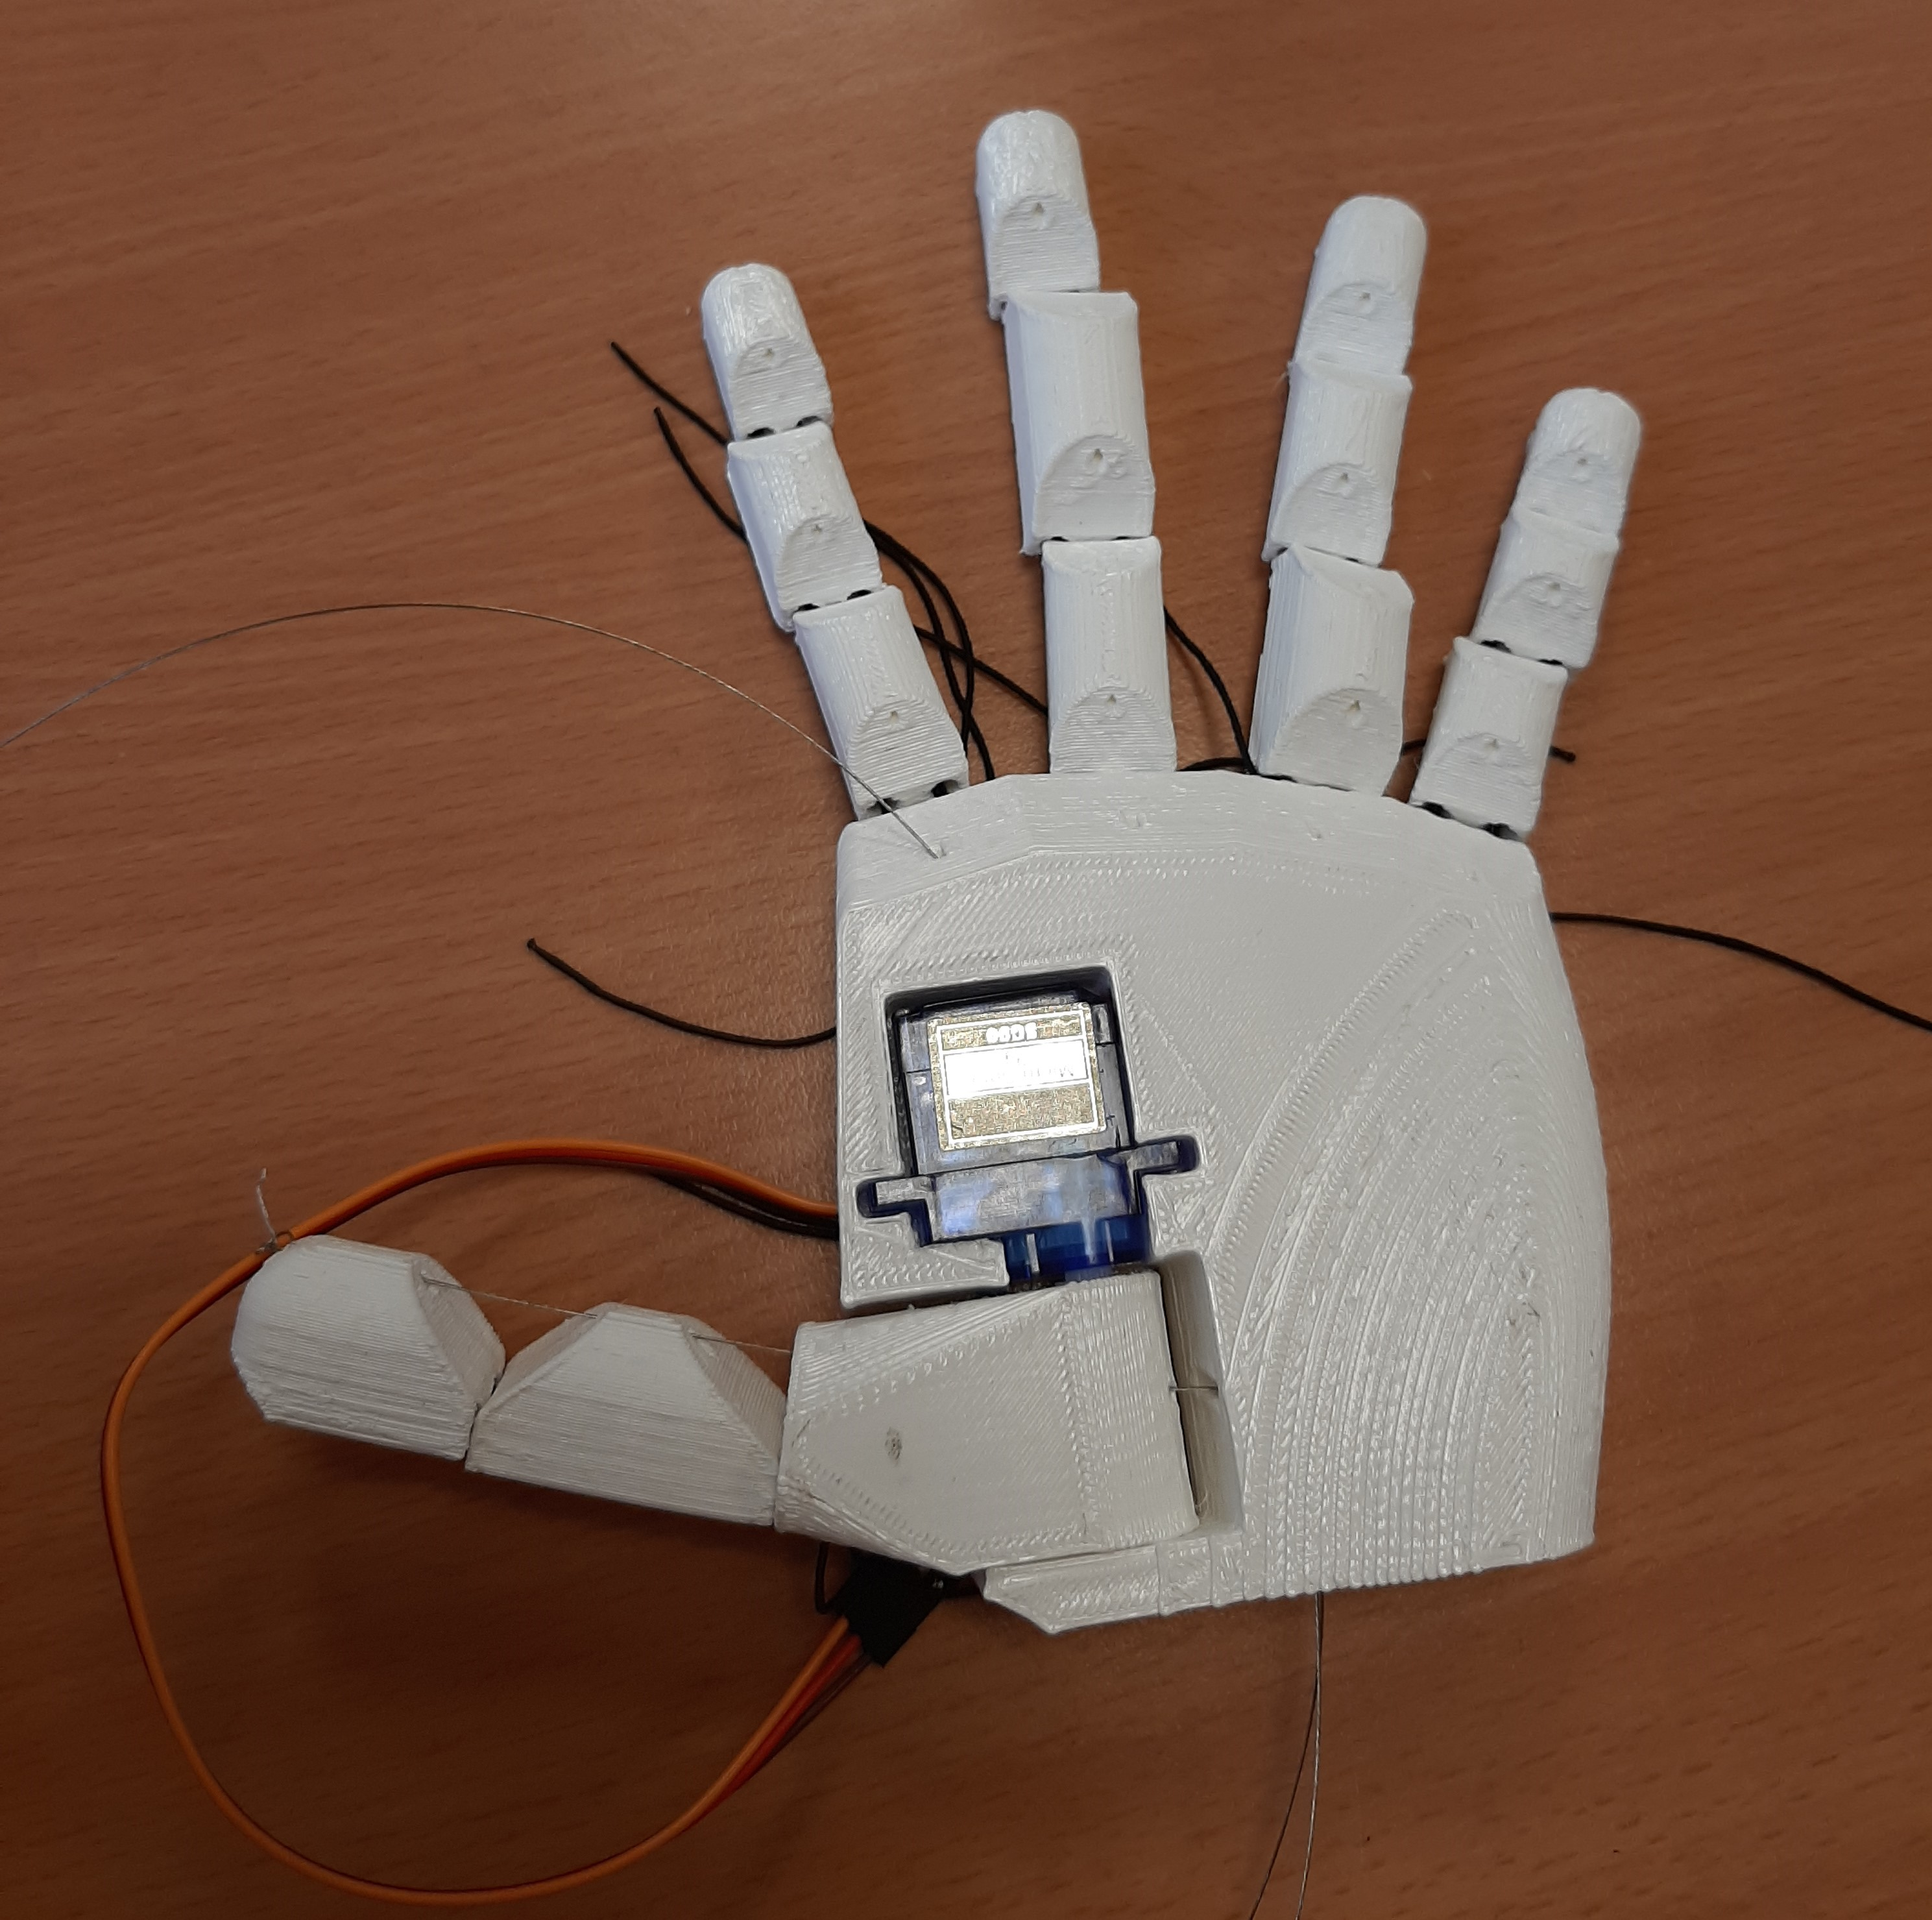
\includegraphics[width=200pt, height=200pt]{Déroulé/Jour_3/Montage de la main/étape2_4.jpg}
    \caption[\'Etape 2]{Montage de la main - \'Etape 2}
    \label{fig:my_label}
\end{figure}

%provisoire
\newpage

\begin{flushleft}
\textbullet \, Visser sur la poulie le petit palonnier en utilisant la petite vis à l'extremité et l'une des grandes au centre :

\begin{figure}[!h]
    \centering
    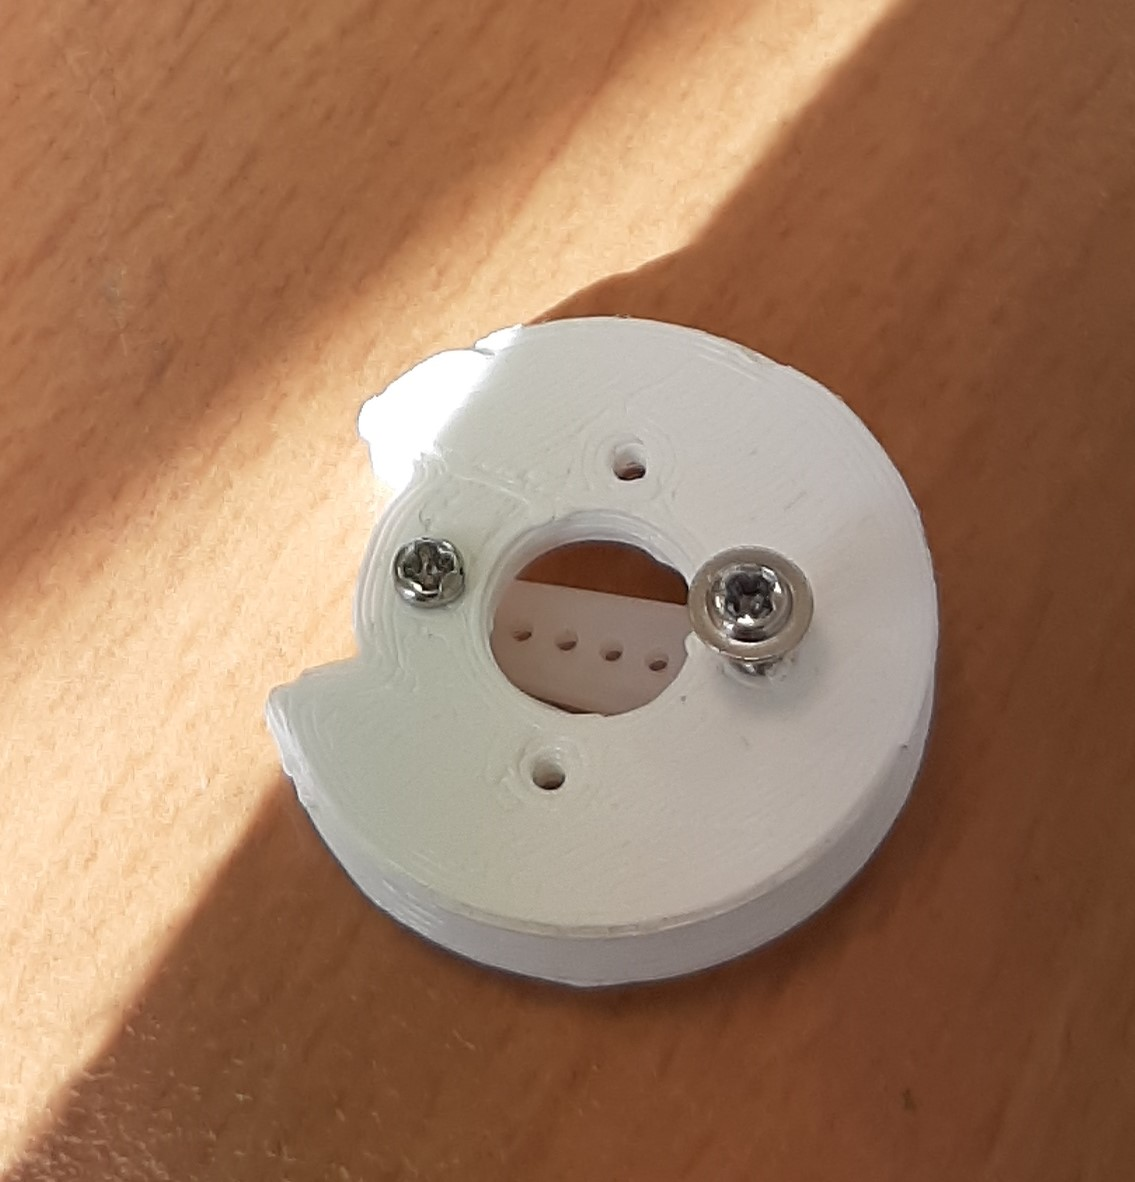
\includegraphics[width=200pt]{Déroulé/Jour_3/Montage de la main/étape3_1.jpg}
    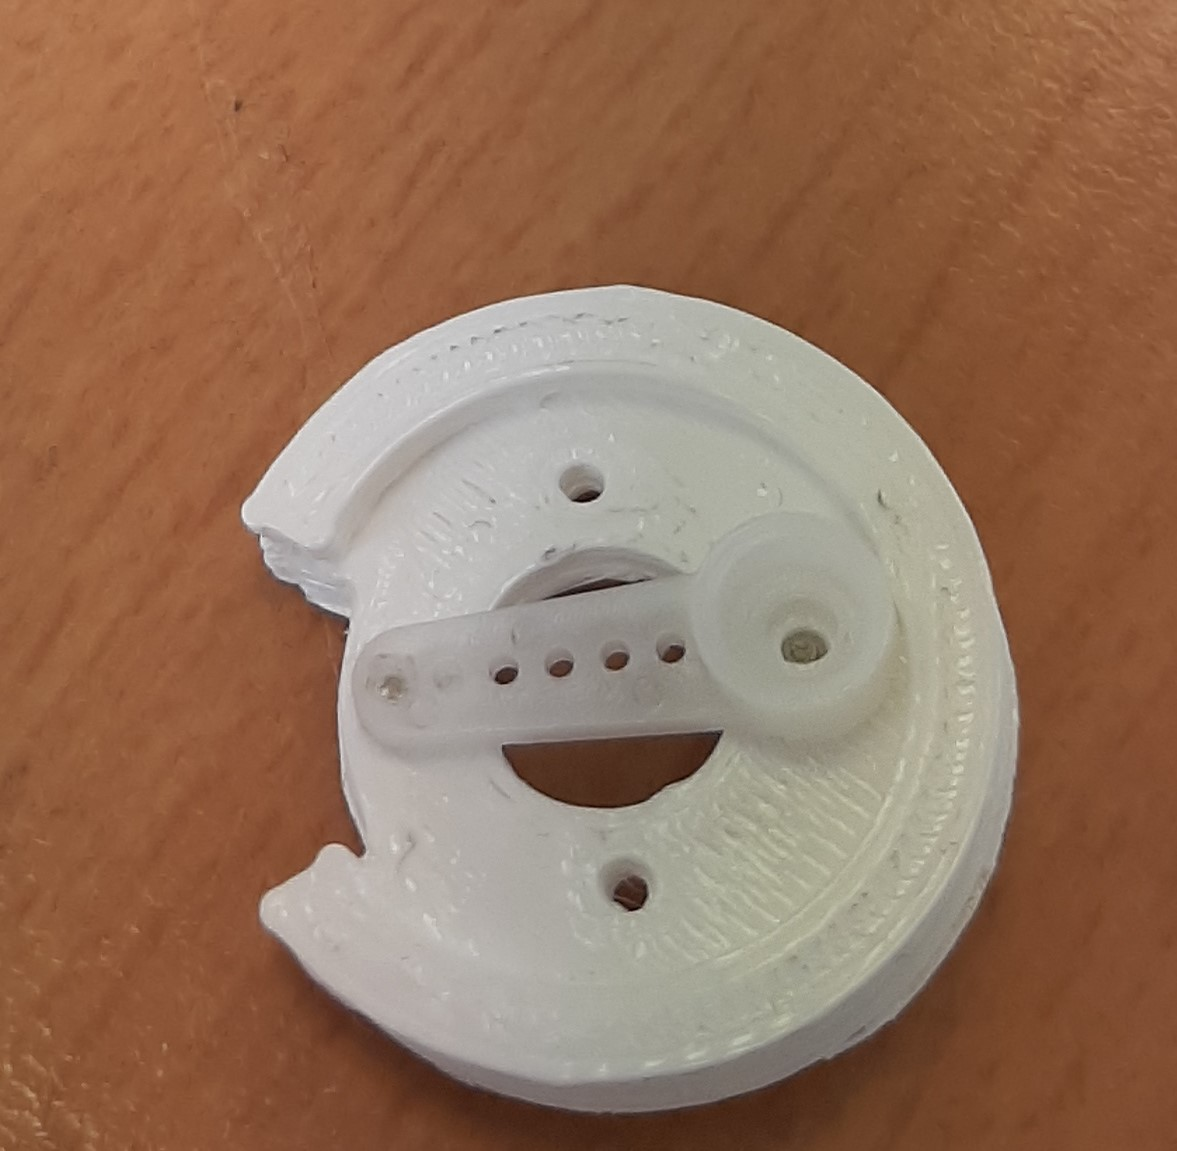
\includegraphics[width=200pt]{Déroulé/Jour_3/Montage de la main/étape3_2.jpg}
    \caption[\'Etape 3]{Montage de la main - \'Etape 3}
    \label{fig:my_label}
\end{figure}

\begin{multicols}{2}
        
\includegraphics[width=60pt,height=60pt]{Déroulé/Jour_1/Manuel d'utilisation/Images/6.jpg}
    
        \columnbreak
    
        \textbf{\large Attention : }\textbf{\textit{ Ne pas visser entièrement la grande vis.}}\\\vspace{0.2cm}
\end{multicols}

\textbullet \, Finir de fixer la grosse vis dans au centre de l'engrenage du servomoteur :

\begin{figure}[!h]
    \centering
    \includegraphics[width=300pt]{Déroulé/Jour_3/Montage de la main/étape4.jpg}
    \caption[\'Etape 4]{Montage de la main - \'Etape 4}
    \label{fig:my_label}
\end{figure}

\begin{multicols}{2}
        \includegraphics[width=60pt,height=60pt]{Déroulé/Jour_1/Manuel d'utilisation/Images/6.jpg}
    
        \columnbreak
    
        \textbf{\large Attention : }\textbf{\textit{ Les servomoteurs que nous utilisons ont une course de 180°, il faut donc positionner correctement le palonnier avant de visser pour ne pas faire forcer le servomoteur lors du fonctionnement.}}\\\vspace{0.2cm}
\end{multicols}

\textbullet \, Fixer les servomoteurs sur le support. Pour cela utiliser la grand vis restante dans le sachet du servomoteur. Des trous sont présents sur le support :

\begin{figure}[!h]
    \centering
    \includegraphics[width=300pt]{Déroulé/Jour_3/Montage de la main/étape5.jpg}
    \caption[\'Etape 5]{Montage de la main - \'Etape 5}
    \label{fig:my_label}
\end{figure}

%provisoire
\newpage

\textbullet \, Fixer le support à l'intérieur de l'avant bras, enrouler les câbles des doigts au niveau des poulies et câbler les potentiomètres et les servomoteurs sur votre breadboard et votre carte :

\begin{figure}[!h]
    \centering
    \includegraphics[width=300pt]{Déroulé/Jour_3/Montage de la main/étape6.jpg}
    \caption[\'Etape 6]{Montage de la main - \'Etape 6}
    \label{fig:my_label}
\end{figure}

\end{flushleft}

%provisoire
\newpage

\subsection{Programmation du code}

\subsubsection{Quels outils utiliser?}

\begin{flushleft}
Lorsque l'on ne souhaite pas s'initier à la programmation à proprement parler, il est possible d'utiliser Tinkercad pour créer ses programmes en passant par des algorithmes. Par ailleurs Tinkercad permet aussi de simuler vos montages pour être sûr qu'ils fonctionneront correctement lorsque vous les réaliserez avec votre carte.\vspace{0.2cm}
\end{flushleft}

\begin{flushleft}
\textbullet \, Se rendre sur le site : \url{https://www.tinkercad.com/} et cliquer sur \textit{Rejoindre maintenant} :
\end{flushleft}

\begin{figure}[!h]
    \centering
    \includegraphics[width=475pt,height=150pt]{Déroulé/Jour_3/configuration Tinkercad/étape1.PNG}
    \caption{Configuration Tinkercad - \'Etape 1}
    \label{fig:my_label}
\end{figure}

\begin{flushleft}
\textbullet \, Une fois votre compte créé, cliquer sur \textit{Circuits} :
\begin{figure}[!h]
    \centering
    \includegraphics[width=150pt,height=150pt]{Déroulé/Jour_3/configuration Tinkercad/étape2.PNG}
    \caption[\'Etape 2]{Configuration Tinkercad - \'Etape 2}
    \label{fig:my_label}
\end{figure}

%provisoire
\newpage

\textbullet \, Cliquer sur \textit{Créer un ciruit} :
\begin{figure}[!h]
    \centering
    \includegraphics[width=150pt,height=100pt]{Déroulé/Jour_3/configuration Tinkercad/étape3.PNG}
    \caption[\'Etape 3]{Configuration Tinkercad - \'Etape 3}
    \label{fig:my_label}
\end{figure}

\textbullet \, Cliquer sur la petite flèche :
\begin{figure}[!h]
    \centering
    \includegraphics[width=450pt,height=100pt]{Déroulé/Jour_3/configuration Tinkercad/étape4.PNG}
    \caption[\'Etape 4]{Configuration Tinkercad - \'Etape 4}
    \label{fig:my_label}
\end{figure}

\textbullet \, Aller dans \textit{Kits de démarrage}, sélectionner \textit{Arduino} et choisir la \textit{Platine d'essai} :
\begin{figure}[!h]
    \centering
    \includegraphics[width=200pt,height=250pt]{Déroulé/Jour_3/configuration Tinkercad/étape5.PNG}
    \caption[\'Etape 5]{Configuration Tinkercad - \'Etape 5}
    \label{fig:my_label}
\end{figure}

%provisoire
\newpage

\textbullet \, Déposer la platine d'essai sur la surface de travail :
\begin{figure}[!h]
    \centering
    \includegraphics[width=300pt,height=125pt]{Déroulé/Jour_3/configuration Tinkercad/étape6.PNG}
    \caption[\'Etape 6]{Configuration Tinkercad - \'Etape 6}
    \label{fig:my_label}
\end{figure}
\end{flushleft}

\begin{flushleft}
Pour programmer la main il est indispensable d'avoir le logiciel Arduino IDE installé sur son ordinateur. Pour ce faire :\vspace{0.4cm}

\textbullet \, Se rendre sur le site : \url{https://www.arduino.cc/}\vspace{0.2cm}

\textbullet \, Aller sur \textit{SOFTWARE} et cliquer sur \textit{DOWNLOADS}

\begin{figure}[!h]
    \centering
    \includegraphics{Déroulé/Jour_3/Installation Arduino IDE/étape1.PNG}
    \caption{Installation Arduino IDE - \'Etape 1}
    \label{fig:my_label}
\end{figure}

%provisoire
\newpage

\textbullet \,  Sélectionner la version correspondant à votre ordinateur :
\begin{figure}[!h]
    \centering
    \includegraphics[width=450pt]{Déroulé/Jour_3/Installation Arduino IDE/étape2.PNG}
    \caption[\'Etape 2]{Installation Arduino IDE - \'Etape 2}
    \label{fig:my_label}
\end{figure}
\end{flushleft}

\subsubsection{Test des servomoteurs}

\begin{flushleft}
\textbullet \, Retourner sur Tinkercad et ouvrir le fichier créé précèdemment.\vspace{0.2cm}

\textbullet \, Taper \textit{servo} dans la barre de recherche et sélectionner celui ci-dessous :
\begin{figure}[!h]
    \centering
    \includegraphics[width=125pt]{Déroulé/Jour_3/TestServo/étape1.PNG}
    \caption{Test servomoteur - \'Etape 1}
    \label{fig:my_label}
\end{figure}

%provisoire
\newpage

\textbullet \, Une fois le servomoteur déposé sur la surface de travail, cliquer sur la petit équerre jusqu'à ce qu'il ait effectué un demi tour sur lui même :
\begin{figure}[!h]
    \centering
    \includegraphics[width=350pt]{Déroulé/Jour_3/TestServo/étape2.PNG}
    \caption[\'Etape 2]{Test servomoteur - \'Etape 2}
    \label{fig:my_label}
\end{figure}

\textbullet \, Ensuite, relier les différents ports du servomoteur comme ci-dessous :
\begin{figure}[!h]
    \centering
    \includegraphics[width=200pt,height=250pt]{Déroulé/Jour_3/TestServo/étape3.PNG}
    \caption[\'Etape 3]{Test servomoteur - \'Etape 3}
    \label{3.18}
\end{figure}

%provisoire
\newpage

\textbullet \, Cliquer sur \textit{Code} :
\begin{figure}[!h]
    \centering
    \includegraphics[height=240pt]{Déroulé/Jour_3/TestServo/étape4.PNG}
    \caption[\'Etape 4]{Test servomoteur - \'Etape 4}
    \label{fig:my_label}
\end{figure}

\textbullet \, Aller dans \textit{Blocs + texte}, \textit{Contrôle} cliquer sur \textit{Totaliser..} et déposer le bloc dans l'espace de travail :\\
De nouvelles choses apparaissent sur la portion de l'écran comportant le code
\begin{figure}[!h]
    \centering
    \includegraphics[width=500pt]{Déroulé/Jour_3/TestServo/étape5.PNG}
    \caption[\'Etape 5]{Test servomoteur - \'Etape 5}
    \label{fig:my_label}
\end{figure}

%provisoire
\newpage

\textbullet \, Cliquer sur \textit{i}, \textit{Renommer la variable} et l'appeler \textit{"pos"} :
\begin{figure}[!h]
    \centering
    \includegraphics[width=250pt,height=100pt]{Déroulé/Jour_3/TestServo/étape6.PNG}
    \caption[\'Etape 6]{Test servomoteur - \'Etape 6}
    \label{fig:my_label}
\end{figure}

\textbullet \, Retourner dans \textit{Sortie}, cliquer sur \textit{Faire pivoter..} et déposer le bloc dans l'espace de travail :
\begin{figure}[!h]
    \centering
    \includegraphics[width=450pt]{Déroulé/Jour_3/TestServo/étape7.PNG}
    \caption[\'Etape 7]{Test servomoteur - \'Etape 7}
    \label{fig:my_label}
\end{figure}

\textbullet \, Retourner dans \textit{Contrôle}, cliquer sur \textit{Patienter} et déposer le bloc dans l'espace de travail :
\begin{figure}[!h]
    \centering
    \includegraphics[width=500pt,height=150pt]{Déroulé/Jour_3/TestServo/étape8.PNG}
    \caption[\'Etape 8]{Test servomoteur - \'Etape 8}
    \label{fig:my_label}
\end{figure}

%provisoire
\newpage

\textbullet \, Faire un clic droit sur l'ensemble de blocs, cliquer sur \textit{Dupliquer} et venir positionner le nouveau bloc sous le précédent :
\begin{figure}[!h]
    \centering
    \includegraphics[width=475pt]{Déroulé/Jour_3/TestServo/étape9.PNG}
    \caption[\'Etape 9]{Test servomoteur - \'Etape 9}
    \label{fig:my_label}
\end{figure}

\textbullet \, Modifier les valeurs des blocs comme ci-dessous, voici le code final pour tester le fonctionnement du servomoteur :
\begin{figure}[!h]
    \centering
    \includegraphics[width=250pt]{Déroulé/Jour_3/TestServo/étape10.PNG}
    \includegraphics[width=200pt]{Déroulé/Jour_3/TestServo/étape10_1.PNG}
    \caption[\'Etape 10]{Test servomoteur - \'Etape 10}
    \label{fig:my_label}
\end{figure}

%provisoire
\newpage

\textbullet \, Copier/coller votre code dans le logiciel Arduino IDE :\\
Il n'est pas possible de le faire sur Tinkercad lorsque l'on écrit un programme en blocs, il faut donc penser à remplacer les valeurs \textit{0} et \textit{90} par la variable \textit{"pos"}, ainsi qu'enlever la plage de valeur de déplacement du servomoteur qui est optionnelle et ne nous intéresse pas ici.
\begin{figure}[!h]
    \centering
    \includegraphics[height=350pt]{Déroulé/Jour_3/TestServo/étape11.PNG}
    \caption[\'Etape 11]{Test servomoteur - \'Etape 11}
    \label{fig:my_label}
\end{figure}

\textbullet \, Effectuer les branchements du servomoteur sur votre carte Arduino (Se référer à la figure \ref{3.18}).\\

%provisoire
\newpage

\textbullet \, Brancher la carte Arduino à l'ordinateur puis cliquer sur \textit{Téléverser} :
\begin{figure}[!h]
    \centering
    \includegraphics[height=350pt]{Déroulé/Jour_3/TestServo/étape12.PNG}
    \caption[\'Etape 12]{Test servomoteur - \'Etape 12}
    \label{fig:my_label}
\end{figure}

\begin{multicols}{2}
    \includegraphics[width=80pt,height=80pt]{Déroulé/Jour_1/Manuel d'utilisation/Images/6.jpg}
    
    \columnbreak
    
    \textbf{\large Attention : }\textbf{\textit{Il est possible que vos servomoteurs soient montés à l'envers. Si lorsque vous téléversez le programme sur la carte vous voyez que le servomoteur force, débranchez le, puis inversez le - et le + dans votre programme. Téléversez de nouveau, le servomoteur doit se comporter normalement.}}
\end{multicols}

\end{flushleft}

\newpage
\subsubsection{La main en elle même}

\input{Déroulé/Jour_3/ProgrammationMain/ProgrammationMain}


%---------------------------------------------------------------------------------------------------------------------------------------------------%

%provisoire
\newpage

\section{Performance}

\subsection{Quelle utilité pour cette main robotique?}
\subsubsection{Exprimer son humeur et/ou un mot}

\begin{flushleft}
En effet, il est possible via l'utilisation des potentiomètres de régler les positions de chaque doigt de manière indépendante. Il est donc possible d'exprimer son humeur via des gestes simples du quotidien.\vspace{0.2cm}

\textbf{Quelques exemples :}

Pour faire comme les plongeurs et signaler que tout va bien, il suffit de faire former au Pouce et à l'Index un rond. Par conséquent il suffit de bouger les potentiomètres respectifs de chacun de ces doigts pour réaliser cette forme avec votre main !

Pour signaler un énervement, on peut imaginer qu'un poing fermé serait la bonne traduction de cette humeur. Il suffit donc de tourner au maximum chaque potentiomètre afin que tous les doigts se referment sur la paume de la main.

Pour exprimer une réussite, on peut former le V de la victoire avec l'Index et le majeur. Il suffit donc de rabattre le Pouce, l'Annulaire et l'Auriculaire sur la paume de la main.

\`A vous de trouver d'autres expressions à faire dire à votre main !

\subsubsection{Dire un mot ou une phrase en langue des signes}

Munissez vous d'un dictionnaire de la langue des signes sur internet, et bougez les potentiomètres de sorte à réaliser une expression proche de celle du mot que vous voulez dire. La langue des signes ne se repose que sur les mouvements de la main mais aussi sur un mouvement de bras et une expression de visage? Mouvez votre bras robotique avec votre propre main pour réaliser ces mouvements, ou bien trouvez votre propre manière de les réaliser !

\subsubsection{Jouer à \textit{"Pierre, Papier, Ciseaux"}}

Si vous souhaitez construire ce bras pour jouer à ce jeu, utilisez trois boutons poussoirs plutôt que des potentiomètres, chaque bouton que vous connecterez à la main correspondra à une des trois positions ! Imaginez et rédigez votre propre programme pour commander les différents mouvements.

\end{flushleft}

%provisoire
\newpage

\section{Pour aller plus loin}

\subsection{Comment créer son propre modèle en CAO ?}

\begin{flushleft}
    L’étape suivante va être de modéliser vous même les pièces que vous souhaitez imprimer. Pour cela il faudra vous munir d’un logiciel de CAO. Dans la partie d’introduction à la CAO vous trouverez un lien renvoyant vers une liste de logiciels de CAO, pour la plupart étant gratuits ou possédant une version gratuite.
    
    Pour modéliser vos pièces il vous faut un logiciel, mais vous devez surtout définir les dimensions et la forme de la pièce que vous vouler concevoir. Pour cela il faut prendre en compte certaines contraintes comme l’utilité qu’aura la pièce (Un objet de décoration, une pièce mécanique, une pièce destinée à recevoir en son sein un (ou des) composant(s) électronique(s), etc...), la taille qu'elle devra avoir, etc...
    
    Pour prendre en main les logiciels et de manière générale la CAO, il existe de nombreux tutoriels sur YouTube qui permettent de s'initier étapes par étapes.
\end{flushleft}

\subsection{Comment choisir ses composants électroniques ?}

\begin{flushleft}
    Pour choisir vos composants il est nécessaire de vous renseigner sur leurs dimensions (que votre modèle 3D soit adapté pour accueillir les composants choisis). Il faut également se renseigner sur les caractéristiques techniques (datasheet en anglais), afin de s'assurer qu'elles soient en accord avec l'utilisation souhaitée.
    
    Tout cela se trouve généralement sur le site du fabricant ou le site d'achat du composant. Sinon tapez "datasheet" suivi du nom du composant sur internet.
\end{flushleft}


\subsection{Perspectives d'amélioration}

\begin{flushleft}
    Si vous souhaitez pousser encore plus loin votre expérience, vous pouvez envisager de rendre votre main un peu plus indépendante de votre Arduino en portant votre carte sur une breadboard ou, encore plus ambitieux, vous lancer dans la soudure et la porter sur une plaque de PCB. 
    
    Il est également possible d'essayer de vous rapprocher encore plus du projet de \href{https://www.instructables.com/3D-Printed-Robotic-Hand/}{TechMartian} en essayant de contrôler la main par Bluetooth.
    
    \begin{multicols}{2}
    \includegraphics[width=60pt,height=60pt]{Déroulé/Jour_1/Manuel d'utilisation/Images/6.jpg}
    
    \columnbreak
    
\textbf{\large Attention : }\textbf{\textit{En plus des composants         nécessaires mentionnés en figure \ref{2.1}, il vous faudra investir     dans un module Bluetooth compatible avec la carte Arduino car nous     n'utilisons pas la même que TechMartian, et il faudra également        modifier le programme Arduino.}}\\
\end{multicols}

Il est également envisageable de décider de modéliser son propre robot via un logiciel, pour concevoir un robot complet. De nouvelles contraintes se présenteront alors, différentes de celles que nous avons rencontré lors de ce projet.

Nous n'avons ici présenté que certains exemples d'améliorations à apporter, mais il en existe sans doute bien d'autres ! \`A vous de réfléchir à celles qui vous intéressent et à la manière dont vous souhaitez les mettre en place. 
\end{flushleft}





\end{document}